% Author Alfredo Sánchez Alberca (asalber@ceu.es)

\newproblem{des-1}{far}{}
%ENUNCIADO
{Se realizó una encuesta a 40 personas de más de 70 años sobre el número de medicamentos distintos que tomaban habitualmente. El resultado de dicha encuesta fue el siguiente:
\begin{center}
3 -- 1 -- 2 -- 2 -- 0 -- 1 -- 4 -- 2 -- 3 -- 5 -- 1 -- 3 -- 2 -- 3 -- 1 -- 4 -- 2 -- 4 -- 3 -- 2 \\
3 -- 5 -- 0 -- 1 -- 2 -- 0 -- 2 -- 3 -- 0 -- 1 -- 1 -- 5 -- 3 -- 4 -- 2 -- 3 -- 0 -- 1 -- 2 -- 3
\end{center}
Se pide:
\begin{enumerate}
\item Obtener la distribución de frecuencias de la muestra.
\item Dibujar el diagrama de barras y el polígono de frecuencias asociados.
\item Dibujar el diagrama de frecuencias acumuladas.
\item Calcular la media aritmética, la mediana y la moda.
\item Calcular la varianza y la desviación típica.
\item Calcular el coeficiente de variación de Pearson.
\end{enumerate}
}
%SOLUCIÓN
{\begin{enumerate}[start=4]
\item $ \bar{x} = 2.225$ medicamentos, $Med =2$ medicamentos y $Mod= 2$ y $3$ medicamentos.
\item $s^2 = 1.974$ medicamentos$^2$, $s= 1.405$ medicamentos.
\item $cv = 0.632$, lo que indica que la hay una dispersión moderada-alta.
\end{enumerate}
}
%RESOLUCIÓN
{}


\newproblem{des-2}{far}{}
%ENUNCIADO
{En un hospital se realizó un estudio sobre el número de personas que ingresaron en urgencias en el mes de noviembre. Los datos observados fueron:
\begin{center}
15 -- 23 -- 12 -- 10 -- 28 -- 7 -- 12 -- 17 -- 20 -- 21 -- 18 -- 13 -- 11 -- 12 -- 26 \\
30 -- 6 -- 16 -- 19 -- 22 -- 14 -- 17 -- 21 -- 28 -- 9 -- 16 -- 13 -- 11 -- 16 -- 20
\end{center}
Se pide:
\begin{enumerate}
\item  Obtener una distribución de frecuencias agrupadas.
\item  Dibujar el histograma y el polígono de frecuencias correspondientes.
\item  Calcular la media aritmética, la mediana y la moda.
\item  Calcular la varianza y la desviación típica.
\item  Calcular el coeficiente de variación de Pearson.
\item  Calcular el tercer decil.
\item  Calcular el percentil 62.
\end{enumerate}
}
%SOLUCIÓN
{
Agrupando en las clases $(5,10]$, $(10,15]$, $(15,20]$, $(20,25]$, $(25,30]$.
\begin{enumerate}[start=3]
\item $ \bar{x} = 16.67$ ingresos, $Med =16.11$ ingresos y $Mod= (10,15]$ y $(15,20]$ ingrsos.
\item $s^2 = 36.75$ ingresos$^2$, $s= 6.06$ ingresos.
\item $cv = 0.365$, lo que indica que hay poca dispersión. 
\item $D_3=12.78$ ingresos.
\item $P_{62}=18.1$ ingresos.
\end{enumerate}
}
%RESOLUCIÓN
{}


\newproblem{des-3}{fis}{*}
%ENUNCIADO
{El número de lesiones padecidas durante una temporada por cada jugador de un equipo de fútbol fue el siguiente:
\begin{center}
0 -- 1 -- 2 -- 1 -- 3 -- 0 -- 1 -- 0 -- 1 -- 2 -- 0 -- 1 \\
1 -- 1 -- 2 -- 0 -- 1 -- 3 -- 2 -- 1 -- 2 -- 1 -- 0 -- 1
\end{center}
Se pide:
\begin{enumerate}
\item Construir la tabla de frecuencias.
\item Dibujar el polígono de frecuencias.
\item Calcular los cuartiles y el rango intercuartílico e interpretarlo.
\item Calcular el coeficiente de asimetría e interpretarlo.
\end{enumerate}
}
%SOLUCIÓN
{\begin{enumerate}[start=3]
\item $C_1 = 0.5$ lesión, $C_2=1$ lesiones y $C_3=2$ lesiones. $RI=1.5$ lesiones, lo que indica que hay bastante dispersión central.
\item $\bar{x}= 1.125$ lesiones, $s^2= 0.776$ lesiones$^2$, $s= 0.88$ lesiones y $g_1=0.49$ lo que indica que la distribución es un poco asimétrica a la derecha.
\end{enumerate}
}
%RESOLUCIÓN
{}


\newproblem{des-4}{gen}{}
%ENUNCIADO
{La siguiente tabla expresa la distribución de las puntuaciones obtenidas por un grupo de alumnos:
\[
\begin{tabular}{|c|c|c|c|c|c|c|c|c|c|}
\hline
0-10 & 10-20 & 20-30 & 30-40 & 40-50 & 50-60 & 60-70 & 70-80 & 80-90 & 90-100
\\ \hline
7 & 8 & 13 & 6 & 7 & 6 & 6 & 5 & 6 & 2 \\ \hline
\end{tabular}
\]
Se pide:
\begin{enumerate}
\item  Dibujar el histograma y polígono de frecuencias.
\item  Calcular la media aritmética, la mediana y la moda.
\item  Calcular el percentil 92.
\item  Calcular la desviación típica.
\item  Calcular el coeficiente de asimetría.
\item  Calcular del coeficiente de curtosis.
\end{enumerate}
}
%SOLUCIÓN
{
\begin{enumerate}[start=2]
\item $ \bar{x} = 42.42$ puntos, $Med =38.3$ puntos y $Mod= (20,30]$ puntos.
\item $P_{92}=84.53$ puntos.
\item $s^2 = 695$ puntos$^2$, $s= 26.36$ puntos.
\item $g_1 = 0.335$, que indica que la distribución es un poco asimétrica hacia la derecha.
\item $g_2 = -1.06$, que indica que la distribución es bastante platicúrtica.
\end{enumerate}
}
%RESOLUCIÓN
{}


\newproblem{des-5}{amb}{}
%ENUNCIADO
{Con el fin de realizar un estudio sobre el aprovechamiento de la energía solar, se han contabilizado las horas de sol registradas durante el mes de enero en las estaciones meteorológicas españolas.
Los datos obtenidos son los siguientes:
\[
\begin{tabular}{|l|c|}
\hline
Horas de Sol & N$^o$ de estaciones \\ \hline\hline
De 50 a 70 & 2 \\ \hline
De 70 a 90 & 6 \\ \hline
De 90 a 110 & 12 \\ \hline
De 110 a 130 & 12 \\ \hline
De 130 a 150 & 16 \\ \hline
De 150 a 170 & 18 \\ \hline
De 170 a 190 & 10 \\ \hline
De 190 a 210 & 2 \\ \hline
De 210 a 230 & 2 \\ \hline
De 230 a 250 & 2 \\ \hline
\end{tabular}
\]
Hallar la media de horas de sol habidas en dicho mes, la desviación típica y el coeficiente de asimetría e interpretarlos.
}
%SOLUCIÓN
{
$\bar x= 140$ horas, $s^2 = 1480$ horas$^2$ y $s= 38.47$ horas, lo que indica que hay poca dispersión y la media es bastante representativa. $g_1=0.226$, lo que indica que la distribución es un poco asimétrica hacia la derecha.
}
%RESOLUCIÓN
{}


\newproblem{des-6}{med}{}
%ENUNCIADO
{En un hospital se ha tomado nota de la concentración de anticuerpos de inmunoglobulina M en el suero sanguíneo de personas sanas, y han resultado los siguientes datos por litro.
Entre paréntesis figura el sexo de la persona (H para hombre y M para mujer).
\begin{center}
\begin{tabular}{lllll}
(H) 1.071 & (H) 0.955 & (H) 0.730 & (M) 0.908 & (M) 0.859  \\
(H) 0.927 & (M) 0.962 & (M) 1.543 & (H) 1.094 & (M) 0.847  \\
(H) 1.214 & (M) 1.456 & (M) 1.516 & (M) 1.002 & (M) 0.799  \\
(M) 0.881 & (M) 1.096 & (M) 0.964 & (H) 0.973 & (H) 1.222  \\
(H) 0.887 & (H) 1.022 & (M) 0.881 & (M) 1.420 & (M) 1.205  \\
(M) 0.822 & (M) 0.920 & (M) 0.544 & (H) 1.254 & (H) 2.048  \\
(M) 1.053 & (M) 0.673 & (M) 1.454 & (H) 1.160 & (H) 1.327  \\
(M) 1.005 & (H) 1.017 & (M) 0.806 & (H) 1.337 & (H) 0.926  \\
(M) 1.029 & (H) 1.516 & (M) 1.231 & (H) 1.249 & (M) 1.627  \\
(M) 1.081 & (H) 1.416 & (M) 1.033 & (M) 1.417 & (M) 1.031  \\
\end{tabular}
\end{center}
Se pide
\begin{enumerate}
\item Construir la tabla de frecuencias desde 0.5 en clases de amplitud 0.1.
\item Dibujar el histograma de frecuencias relativas y frecuencias relativas acumuladas.
\item ¿En qué población es más representativa la media, en la de hombres o en la de mujeres?
\end{enumerate}
}
%SOLUCIÓN
{Llamando $X$ a la concentración de inmunoglobulina en hombres e $Y$ a la concentración en mujeres:
\begin{enumerate}[start=3]
\item $\bar x = 1.175$, $s_x = 0.284$, $cv_x=0.24$, $\bar y=1.077$, $s_y=0.279$, $cv_y=0.26$, lo que indica que hay una poca menos dispersión en los hombres y su media es un poco más representativa. 
\end{enumerate}
}
%RESOLUCIÓN
{}


\newproblem{des-7}{med}{*}
%ENUNCIADO
{En un estudio sobre el crecimiento se tomaron dos muestras, una de niños recién nacidos y otra de niños con un año de edad. Las estaturas observadas en cada muestra fueron:
\begin{quote}
Recién nacidos: 51-50-51-53-49-50-53-50-47-50.\\
Niños de un año: 62-65-69-71-65-66-68-69.
\end{quote}

¿Según el coeficiente de variación, en cuál de las dos muestras es más representativa la media?
}
%SOLUCIÓN
{Llamando $X$ a las estaturas de los niños recién nacidos e $Y$ a las estaturas de los niños de 1 año: 
$\bar x = 50.4$ cm, $s_x = 1.685$ cm, $cv_x=0.034$, $\bar y=66.875$ cm, $s_y=2.713$ cm, $cv_y=0.041$, lo que indica que ambas medias son muy representativas pero un poco más la de los niños recién nacidos.  
}
%RESOLUCIÓN
{Llamemos $X$ a las estaturas de los niños recién nacidos e $Y$ a las estaturas de los niños de 1 año. 
La media muestral es tanto más representativa cuanto más pequeño es el coeficiente de variación.
Por tanto, para ver en qué muestra es más representativa la media, tenemos que comparar los coeficientes de correlación de ambas muestras.
El coeficiente de correlación esta definido por la fórmula
\[
cv=\frac{s}{\bar{x}},
\]
de modo que, para calcular los coeficientes de variación tenemos que calcular la media y la desviación típica de cada muestra. 
Llamando $X_{1}$ a la talla de los recién nacidos y $X_{2}$ a la talla de los niños de un año, tenemos
\begin{eqnarray*}
\bar{x} & = & \frac{\sum_{i}^{}x_{i}}{n_{x}} =
\frac{51+50+\cdots +50}{10} = \frac{504}{10} =50.4 \mbox{cm}, \\
s_{x}^2 & = & \frac{\sum_{i}^{}x_{i}^2}{n_{x}}-\bar{x}^2 =
\frac{51^2+50^2+\cdots 50^2}{10}-50.4^2 = 2543-2540.16 = 2.84 \mbox{cm}^2,  \\
s_{x} & = & \sqrt{2.84} = 1.69 \mbox{cm},  \\
\bar{y} & = & \frac{\sum_{i}^{}y_{i}}{n_{y}} =
\frac{62+65+\cdots +69}{8} = \frac{535}{8} = 66.875 \mbox{cm},  \\
s_{y}^2 & = & \frac{\sum_{i}^{}y_{i}^2}{n_{y}}-\bar{y}^2 =
\frac{62^2+65^2+\cdots 69^2}{8}-66.875^2 = 4479.625-4472.266 = 7.36 \mbox{cm}^2,  \\
s_{y} & = & \sqrt{7.36} = 2.713 \mbox{cm}.  \\
\end{eqnarray*}
Sustituyendo ahora en la fórmula del coeficiente de variación obtenemos
\[ 
cv_{x}=\frac{s_{x}}{\bar{x}} = \frac{1.69}{50.4} = 0.034 \qquad
cv_{y}=\frac{s_{y}}{\bar{y}} = \frac{2.713}{66.875} = 0.041.
\]
En consecuencia, como $cv_{x}<cv_{y}$, la media es más representativa en la muestra de niños recien nacidos.
}


\newproblem*{des-8}{amb}{}
%ENUNCIADO
{Las temperaturas medias mensuales (en $^\circ$C) durante el año 2001 en Madrid y Sevilla fueron:
\begin{center}
\begin{tabular}{|l|r|r|r|r|r|r|r|r|r|r|r|r|}
\hline
Ciudad &    Ene &    Feb &    Mar &    Abr &    May &    Jun &    Jul &    Ago &    Sep &    Oct &    Nov &    Dic \\
\hline
 Madrid                  &  $7.2$ &  $8.4$ & $12.2$ & $13.7$ & $16.7$ & $23.3$ & $24.2$ & $25.5$ & $20.4$ & $16.2$ &  $8.1$ &  $4.2$ \\
\hline
 Sevilla                 & $12.1$ & $13.6$ & $16.8$ & $19.0$ & $20.9$ & $27.0$ & $26.6$ & $28.2$ & $24.7$ & $21.3$ & $13.8$ & $11.5$ \\
\hline
\end{tabular}
\end{center}
¿En cuál de la dos ciudades ha habido una mayor variación de temperatura?
}


\newproblem*{des-9}{amb}{}
%ENUNCIADO
{El siguiente diagrama muestra los datos de una muestra de consumo de energía primaria en la industria española durante el año 2002.
\[
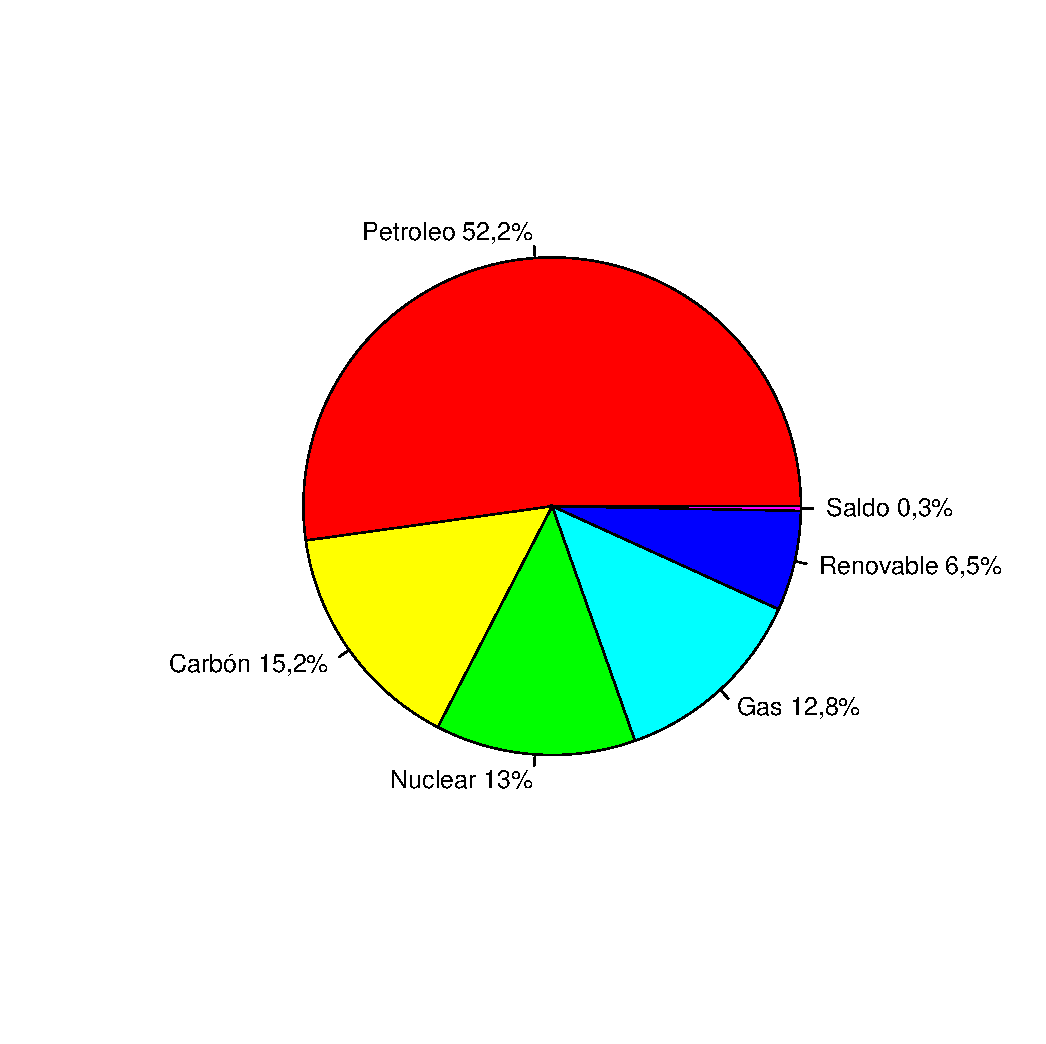
\includegraphics[scale=0.5]{img/energias-des-9}
\]
Realizar un estudio descriptivo de los datos que incluya todos los estadísticos posibles.
}


\newproblem{des-10}{gen}{*}
%ENUNCIADO
{El siguiente diagrama refleja el porcentaje de calificaciones obtenidas en un examen realizado a 80 alumnos:
\[
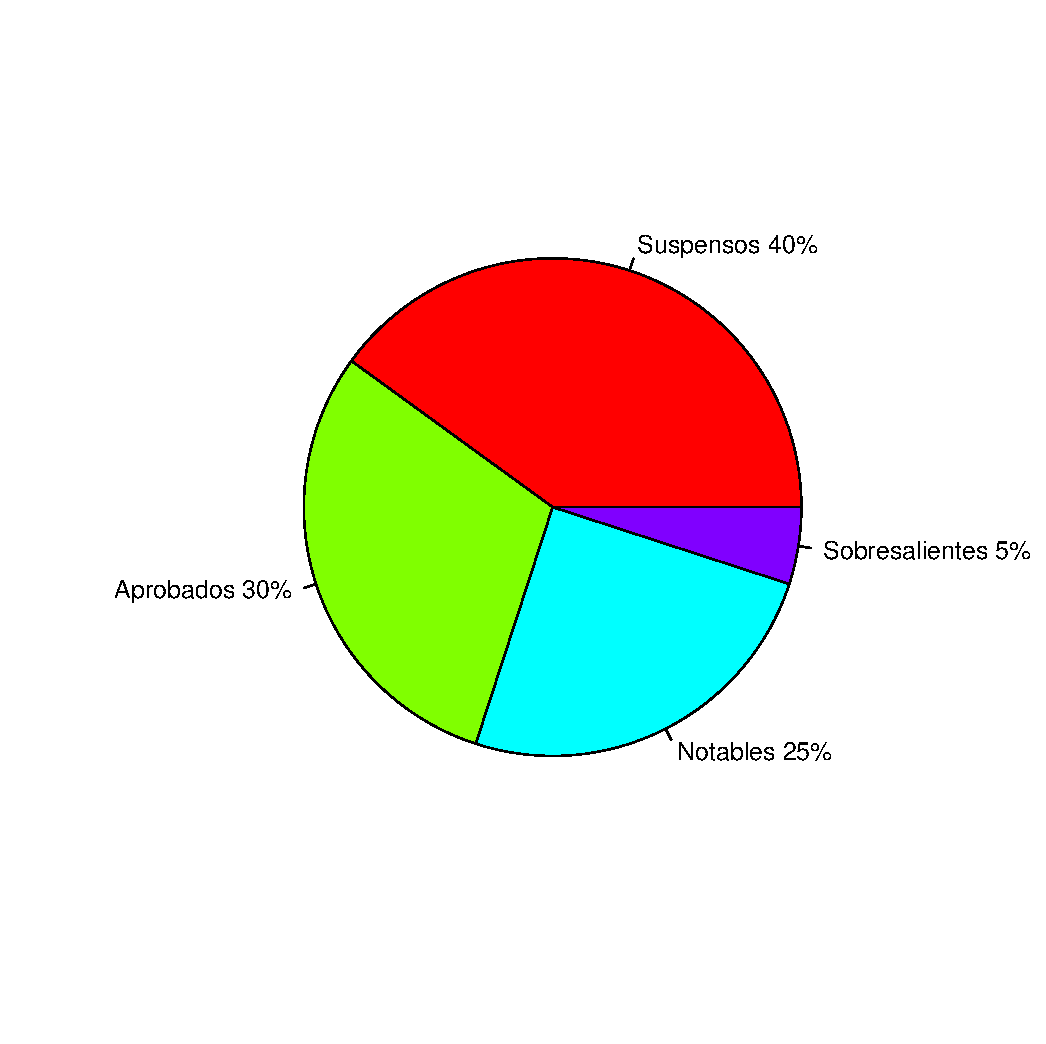
\includegraphics[scale=0.5]{img/sectores-des-10}
\]
Se pide:
\begin{enumerate}
\item Construir la tabla de frecuencias para las calificaciones.
\item Dibujar el polígono de frecuencias acumuladas.
\item Calcular todos los estadísticos de tendencia central que sean posibles.
\item A partir de la variable calificación, construir la variable nota con los siguientes intervalos: Suspenso $[0,5)$, Aprobado $[5,7)$, Notable $[7,9)$ y Sobresaliente $[9,10]$, y calcular la nota media y estudiar su representatividad.
\end{enumerate}
Nota: En los tres primeros apartados se debe trabajar con la variable calificación, mientras que en el último debe utilizarse la variable nota.
}
%SOLUCIÓN
{\begin{enumerate}[start=3]
\item $Me=\mbox{Aprobado}$ y $Mo=\mbox{Suspenso}$.
\item $\bar x = 5.275$ puntos, $s=2.447$ puntos y $cv=0.464$, de manera que la media es moderadamente representativa.  
\end{enumerate}
}
%RESOLUCIÓN
{}


\newproblem{des-11}{gen}{*}
%ENUNCIADO
{Sea la variable estadística agrupada en intervalos cuya distribución de frecuencias viene dada por la siguiente tabla:
\[
\begin{tabular}{|c|c|c|c|c|}
\hline
Intervalos & $n_{i}$ & $f_{i}$ & $N_{i}$ & $F_{i}$ \\ \hline
$\left[ 0,10\right) $ & 10 & 0.25 &  &  \\ \hline
$\left[ 10,20\right) $ &  &  & 22 &  \\ \hline
$\left[ 20,30\right) $ &  & 0.30 &  &  \\ \hline
$\left[ 30,40\right) $ &  &  &  &  \\ \hline
\end{tabular}
\]
\begin{enumerate}
\item  Completar la tabla y hallar la desviación típica.
\item  Calcular la mediana y el rango intercuartílico e interpretarlos.
\end{enumerate}
}
%SOLUCIÓN
{\begin{enumerate}
\item $\bar{x}= 18.5$, $s^2=102.75$ y $s=10.14$. 
\item $Med = 18.33$, $C_1=10$, $C_3 = 26.27$ y $RI= 16.17$ lo que indica, teniendo en cuenta que el rango de toda la distribución es 40, que la dispersión es moderada.
\end{enumerate}
}
%RESOLUCIÓN
{}


\newproblem{des-12}{gen}{}
%ENUNCIADO
{Dada la gráfica correspondiente a un polígono acumulativo de frecuencias relativas de una variable estadística agrupada en intervalos de una muestra de tamaño 20:
\[
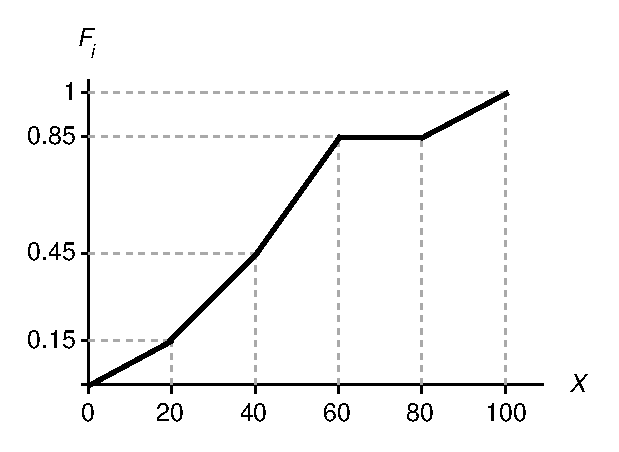
\includegraphics[scale=0.8]{img/poligono-des-12}
\]
se pide:
\begin{enumerate}
\item Construir la tabla de frecuencias.
\item Dibujar el histograma correspondiente.
\item Calcular la mediana y la moda.
\item Calcular la media aritmética y la desviación típica.
\end{enumerate}
}
%SOLUCIÓN
{\begin{enumerate}[start=3]
\item $Med =42.5$ y $Mod= (40,60)$.
\item $\bar = 44$, $s^2 = 564$, $s= 23.75$.
\end{enumerate}
}
%RESOLUCIÓN
{}


\newproblem{des-13}{gen}{*}
%ENUNCIADO
{Dada la siguiente tabla de frecuencias:
\[
\begin{tabular}{|c|c|c|c|c|}
\hline
Intervalos & $n_{i}$ & $f_{i}$ & $N_{i}$ & $F_{i}$ \\ \hline
$\left[ 0,5\right) $ & 2 &  &  &  \\ \hline
$\left[ 5,10\right) $ &  &  & 8 &  \\ \hline
$\left[ 10,15\right) $ &  &  &  & 0.7 \\ \hline
$\left[ 15,20\right) $ & 6 &  &  &  \\ \hline
\end{tabular}
\]
\begin{enumerate}
\item Completar la tabla.
\item Calcular el coeficiente de variación y el rango intercuartílico e interpretar los resultados.
\end{enumerate}
}
%SOLUCIÓN
{$\bar x= 11.5$, $s^2= 24$, $s=4.9$, $cv=0.426$, lo que indica que hay una dispersión moderada. $C_1=7.5$, $C_3=15.83$, $RI=8.33$, lo que indica que la dispersión central también es moderada.
}
%RESOLUCIÓN
{}


\newproblem{des-14}{med}{*}
%ENUNCIADO
{Para obtener información acerca del número de consultas al médico, $X$, que los abonados de una compañía de seguro médico realizan cada mes, trabajando con una muestra de 200 abonados, la distribución de frecuencias fue:
\[
\begin{array}{cc}
\hline
x_i & n_i \\
\hline
0 & 83\\
1 & 51\\
2 & 26\\
3 & 15\\
4 & 9\\
5 & 6\\
6 & 5\\
7 & 3\\
8 & 1\\
9 & 1\\
\hline
\end{array}
\]
Y se pide calcular:
\begin{enumerate}
\item Media, desviación típica y coeficiente de variación del número de visitas al médico. Interpretar el coeficiente de variación.
\item Coeficiente de asimetría de la distribución. Interpretarlo.
\item Percentiles 10 y 90. Interpretarlos.
\end{enumerate}
}
%SOLUCIÓN
{\begin{enumerate}
\item $\bar x=1.41$ consultas, $s^2=3.2919$ consultas$^2$, $s=1.8144$ consultas y $cv=1.29$, lo que indica que hay muchas dispersión y la
media no es muy representativa.
\item $g_1=1.66$ lo cual indica que la distribución es bastante asimétrica hacia la derecha, pero no lo suficiente para considerarla
anormal.
\item $P_{10}=0$ lo que indica que el 10\% de las personas de la muestra que menos consultas realizaron, realizaron 0 consultas, y $P_{90}=4$ lo que indica que el 10\% de las personas de la muestra que más consultas realizaron, realizaron 4 o más consultas.
\end{enumerate}
}
%RESOLUCIÓN
{}


\newproblem{des-15}{med}{*}
%ENUNCIADO
{Los siguientes datos corresponden a 49 mediciones del colesterol HDL (en mg/dl) tomadas en personas de edades y hábitos similares:
\[
\begin{array}{ccccccc}
69.4 & 68.3 & 60.4 & 70.1 & 93.1 & 71.1 & 58.2 \\
73.6 & 70.9 & 71.5 & 57.1 & 58.7 & 56.9 & 74.8 \\
55.6 & 66.6 & 63.7 & 74.5 & 77.3 & 88.0 & 70.3 \\
75.9 & 67.5 & 70.0 & 67.3 & 67.6 & 77.8 & 70.6 \\
64.9 & 68.0 & 85.1 & 72.8 & 61.6 & 69.2 & 69.6 \\
68.1 & 50.1 & 60.2 & 52.0 & 76.4 & 77.2 & 82.4 \\
74.6 & 71.9 & 73.8 & 82.2 & 71.9 & 73.6 & 69.1 \\
\end{array}
\]
\begin{enumerate}
\item Agrupar los datos en 6 clases comenzando en 50 y terminando en $93,2$.
\item Calcular el rango intercuartílico e interpretarlo.
\item Razonar si la media de estos datos es representativa de los mismos.
\end{enumerate}
}
%SOLUCIÓN
{\begin{enumerate}[start=2]
\item $C_1=64.874$ mg/dl, $C_3=75.071$ mg/dl y $RI=10.197$ mg/dl. Esto es bastante menos de la mitad del recorrido de la variable, lo que indica que los datos centrales están bastante concentrados.
\item $\bar x= 69.469$ mg/dl, $s^2=71.952$ (mg/dl)$^2$, $s=8.482$ mg/dl y $cv=0.122$, lo que indica que hay poca dispersión y por tanto la media es muy representativa.
\end{enumerate}
}
%RESOLUCIÓN
{}


\newproblem{des-16}{med}{}
%ENUNCIADO
{Se ha llevado a cabo un estudio sobre el número de radiografías realizadas durante el último año a un grupo de 200 personas, y la información se presenta en la siguiente tabla incompleta:
\[
\begin{array}{|c|c|c|c|}
\hline
\mbox{Radiografías} & \mbox{Personas} & f_i & F_i \\
\hline
0 &    & 0.20 &      \\
1 & 84 &      &      \\
2 &    &      & 0.72 \\
3 &    &      &      \\
4 & 24 &      &      \\
5 &    & 0.02 &      \\  
\hline
\end{array}
\]
\begin{enumerate}
\item Completar tabla.
\item Calcular media, mediana, desviación típica y coeficiente de variación e interpretar los resultados.
\end{enumerate}
}
%SOLUCIÓN
{\begin{enumerate}[start=2]
\item $\bar x= 1.62$ radiografías, $s^2=1.875$ radiografías$^2$, $s=1.37$ radiografías y $cv=0.845$, lo que indica que hay bastante dispersión y la media no es muy representativa.
\end{enumerate}
}
%RESOLUCIÓN
{}


\newproblem{des-17}{far}{*}
%ENUNCIADO
{En un estudio diseñado para investigar la efectividad de un nuevo producto anestésico local, la misma cantidad de producto fue suministrada a 20 pacientes, y se midió el tiempo transcurrido hasta lograr cierto grado de sensibilidad. Los resultados, en minutos, son los siguientes:
\begin{center}
38, 43, 52, 64, 39, 54, 51, 47, 42, 58, 63, 36, 39, 47, 49, 46, 52, 44, 38, 57
\end{center}
\begin{enumerate}
\item Agrupar los datos desde 35 a 65 en 6 clases diferentes.
\item Una vez agrupados, calcular: Media, Desviación Típica y Coeficiente de Asimetría.
\item Teniendo en cuenta la distribución agrupada y suponiendo que todos aquellos datos que se encuentren por arriba del percentil 95 tienen un comportamiento anormal, ¿cuáles de los pacientes se puede considerar que han tenido un tiempo de insensibilidad anormal?
\end{enumerate}
}
%SOLUCIÓN
{\begin{enumerate}[start=2]
\item $\bar x= 47.75$ minutos, $s^2=66.188$ minutos$^2$, $s=8.136$ minutos. $g_1=0.268$ lo que indica que la distribución es ligeramente asimétrica hacia la derecha.
\item $P_{95}=62.5$ minutos. 
\end{enumerate}
}
%RESOLUCIÓN
{}


\newproblem{des-18}{gen}{*}
%ENUNCIADO
{Si a todos los datos de una muestra se les suma una misma cantidad positiva, ¿cómo se ve afectada la representatividad de la media?
¿Y si se multiplican por un mismo número distinto de 0?
Razonar la respuesta.
}
%SOLUCIÓN
{La representatividad de la media aumenta cuando se suma una constante a los datos y se mantiene igual cuando se multiplican por una constante.
}
%RESOLUCIÓN
{Sea $X$ una variable cualquiera y consideremos la variable $Y=X+c$ resultante de sumar una constante $c> 0$ a los valores de $X$. Entonces, aplicando las propiedades de las transformaciones lineales tenemos
\[
cv_{y} = \frac{s_y}{|\bar y|} = \frac{s_x}{|\bar x +c|} < \frac{s_x}{|\bar x|} = cv_{x},
\]
luego al ser menor el coeficiente de variación $Y$ hay menos dispersión relativa y su media es más representativa.

Por otro lado si ahora tomamos $Y=cX$ como la variable resultante de multiplicar los datos de $X$ por una constante $c\neq 0$, tenemos, de nuevo apliando las propiedades de las transformaciones lineales,
\[
cv_{y} = \frac{s_y}{|\bar y|} = \frac{cs_x}{|c\bar x|} = \frac{s_x}{|\bar x|} = cv_{x},
\]
de modo que el coeficiente de variación no se altera y por tanto la representatividad de la media es la misma.
}


\newproblem{des-19}{med}{*}
%ENUNCIADO
{Como parte de un proyecto de investigación, los investigadores obtuvieron los siguientes datos respecto a los niveles de peróxido lípido (en nmol/ml) en el suero de 30 individuos adultos bajo tratamiento de Diabetes Mellitus:
\[
\begin{array}{cccccccccc}
3.09 & 6.06 & 7.34 & 5.32 & 4.29 & 5.36 & 6.01 & 7.84 & 3.87 & 5.23 \\
4.67 & 7.89 & 5.16 & 6.32 & 6.45 & 3.21 & 5.98 & 6.45 & 7.12 & 4.13 \\
5.16 & 3.04 & 4.56 & 5.67 & 5.98 & 6.23 & 7.34 & 5.32 & 4.21 & 7.13 \\
\end{array}
\]
Agrupar los datos en 5 clases de amplitud unidad, comenzando en 3, y sobre la distribución obtenida:
\begin{enumerate}
\item Calcular media, desviación típica y coeficiente de variación de los niveles de peróxido lípido.
Interpretar el coeficiente de variación.
\item Calcular cuartiles de la distribución e interpretarlos.
\item Dibujar el diagrama de caja y bigotes y comprobar si hay o no datos atípicos.
\end{enumerate}
}
%SOLUCIÓN
{\begin{enumerate}
\item $\bar x = 5.667$ nmol/ml, $s^2= 1.668$ (nmol/ml)$^2$, $s= 1.292$ nmol/ml y $cv=0.228$, lo que indica que hay poca dispersión y la media es bastante representativa.
\item $C_1=4.7$ nmol/ml, $C_2=5.667$ nmol/ml y $C_3= 6.75$ nmol/ml.
\item Las vallas son $v_1=1.625$ y $v_2=9.825$. Todos los datos están entre las vallas y no hay datos atípicos. Los bigotes son $b_1=3.04$ nmol/ml y $b_2=7.89$ nmol/ml.
\end{enumerate}
}
%RESOLUCIÓN
{}


\newproblem{des-20}{med}{*}
%ENUNCIADO
{A continuación figura la distribución de edades de una muestra de 65 individuos sujetos a rehabilitación tras un infarto de miocardio:
\begin{center}
\begin{tabular}{|c|c|c|c|c|c|}
\hline
Edad & [40-50) & [50-60) & [60-70) & [70-80) & [80-90)  \\ \hline
$n_i$ & 6 & 12 & 23 & 19 & 5  \\ \hline
\end{tabular}
\end{center}
\begin{enumerate}
\item Sabemos que una distribución normal es simétrica y mesocúrtica.
Por tanto, una primera idea de si los datos muestrales provienen de una distribución normal nos la puede dar ver si estos valores se encuentran en el intervalo [-2, 2].
¿Podríamos suponer según esto que los datos provienen de una distribución normal?
\item Calcular la edad, por encima de la cuál se encuentra el 15\% de los individuos sujetos a rehabilitación tras un infarto de miocardio,
en esta muestra.
\end{enumerate}
}
%SOLUCIÓN
{\begin{enumerate}
\item $\bar x= 65.769$ años, $s^2= 114.823$ años, $s=10.716$ años. $g_1=-0.228$ y $g_2=-0.55$, como tanto el coefiente de asimetría como el de apuntamiento están entre -2 y 2, podemos suponer que los datos provienen de una población normal.
\item $P_{85}=77.5$ años.  
\end{enumerate}
}
%RESOLUCIÓN
{}


\newproblem{des-21}{med}{*}
%ENUNCIADO
{Para obtener información acerca del porcentaje de albúmina en el suero proteico de personas adultas, se analizaron muestras de 32 personas, con los siguientes resultados:
\[
\begin{array}{cccccccc}
70.2 & 63.5 & 65.8 & 67.9 & 60.1 & 69.7 & 64.2 & 65.3 \\
62.8 & 68.4 & 65.2 & 66.3 & 70.7 & 71.8 & 68.7 & 71.9 \\
64.4 & 62.4 & 60.4 & 67.0 & 62.9 & 65.9 & 67.5 & 66.6 \\
67.8 & 70.5 & 63.1 & 65.3 & 69.5 & 71.4 & 61.0 & 64.3 \\
\end{array}
\]
\begin{enumerate}
\item Agrupar la distribución de porcentajes de albúmina en 6 clases de igual amplitud, desde 60 hasta 72.
\item En la distribución agrupada calcular media, desviación típica, y cuartiles.
\item ¿Es representativa la media de la muestra de porcentajes de albúmina?
\item Dibujar el diagrama de caja y bigotes de la distribución y determinar si hay o no algún dato atípico.
\end{enumerate}
}
%SOLUCIÓN
{\begin{enumerate}[start=2]
\item $\bar x=66.3125\%$, $s^2=9.9023\%^2$, $s=3.1468\%$. $C_1=64\%$, $C_2=66\%$, $C_3=69\%$.
\item $cv=0.05$ lo que indica que hay muy poca dispersión y la media es muy representativa.
\end{enumerate}
}
%RESOLUCIÓN
{}


\newproblem*{des-22}{amb}{}
%ENUNCIADO
%CAMBIAR DATOS PARA QUE SALGA MÁS ASIMÉTRICA
{Para determinar la validez de un terreno para un determinado cultivo, se realizó un muestreo sistemático del terreno obteniendo 18 valoraciones del PH del suelo-agua (en relación 1:2.5).
Los valores obtenidos fueron:
\[
\begin{array}{ccccccccc}
5.82 & 6.23 & 6.17 & 7.11 & 6.44 & 6.08 & 6.03 & 5.91 & 6.83 \\
6.55 & 6.24 & 6.12 & 6.32 & 5.86 & 6.64 & 6.73 & 7.24 & 6.02
\end{array}
\]
Se pide:
\begin{enumerate}
\item Calcular el coeficiente de asimetría e interpretarlo.
\item Aplicar una transformación a la variable para obtener otra variable con una simetría más normal.
\end{enumerate}
}


\newproblem{des-23}{far}{}
%ENUNCIADO
{Para determinar la eficacia de un nuevo método para la medición del hematocrito en sangre, se repitió la medida 8 veces sobre una misma muestra de sangre, obteniéndose los siguientes resultados (en porcentaje de hematocrito sobre volumen de plasma sanguíneo):
\[
\begin{array}{cccccccc}
42.2 & 42.1 & 41.9 & 41.8 & 42 & 42.1 & 41.9 & 42.
\end{array}
\]
¿Se puede afirmar que se trata de un buen método de medición?
}
%SOLUCIÓN
{$\bar x= 42\%$, $s^2=0.015\%^2$, $s=0.1225\%$ y $cv=0.003$ lo que indica que la variabilidad entre las mediciones es ínfima y por tanto se trata de un buen método de medición.
}
%RESOLUCIÓN
{Para ver si se trata de un buen método de medición, tenemos que comprobar que entre las sucesivas mediciones no haya grandes diferencias. Se trata, por tanto, de medir la variabilidad de la muestra y para ello calculamos el coeficiente de variación:
\begin{align*}
\bar x & = \frac{\sum x_i}{n} = \frac{42.2+\cdots+42}{8} = \frac{336}{8}= 42\%,\\
s^2 & = \frac{\sum x_i^2}{n}-\bar x^2 = \frac{42.2^2+\cdots+42^2}{8}-42^2 = \frac{14112.12}{8}-42^2= 0.015\%^2,\\
s &= \sqrt{0.015} = 0.1225\%,\\
cv &= \frac{s}{|\bar x|} = \frac{0.1225}{42} = 0.003.
\end{align*}
Como el coeficiente de variación es muy pequeño, podemos concluir que la variabilidad entre las mediciones es ínfima y por tanto se trata de un buen método de medición.
}


\newproblem{des-24}{fis}{}
%ENUNCIADO
{En cuestionario sobre la dependencia de las personas mayores de 75 años se preguntaba sobre la necesidad de ayuda en el desarrollo normal de su vida. Las posibles respuestas eran:
\begin{enumerate}
\item Ninguna ayuda.
\item Ayuda al subir las escaleras.
\item Ayuda al subir las escaleras y al incorporarse de una posición sentada o tumbada.
\item Ayuda al subir las escaleras, al incorporarse, y al vestirse.
\item Ayuda para prácticamente todo.
\end{enumerate}
El cuestionario lo respondieron 20 personas, y los resultado obtenidos fueron
\begin{center}
b -- d -- a -- b -- c -- c -- b -- c -- d -- e -- a -- b -- c -- e -- a -- b -- c -- d -- b -- b
\end{center}
Se pide:
\begin{enumerate}
\item Representar gráficamente la distribución de frecuencias.
\item Calcular las medidas de tendencia central.
\item Calcular los cuartiles y el decil 8.
\item ¿Qué se puede decir sobre la dispersión?
\end{enumerate}
}
%SOLUCIÓN
{\begin{enumerate}[start=2]
\item $Me$ ente b y c y $Mo=b$. 
\item $C_1=$b, $C_2$ entre b y c, $C_3=$ entre c y d, $D_8=d$.
\item Suponiendo que hay la misma distancia entre categorías y asignando rangos a cada valor ($a=1,b=2,c=3,d=4,e=5$), tenemos $\bar x=2.7$, $s^2=1.41$, $s=1.187$ y $cv=0.44$, lo que indica una dispersión moderada. 
\end{enumerate}
}
%RESOLUCIÓN
{}


\newproblem{des-25}{amb}{*}
%ENUNCIADO
{Como parte de un proyecto de investigación, los investigadores obtuvieron los siguientes datos respecto a los niveles (en partes por millón) de cierto contaminante químico en 30 suelos diferentes de la Comunidad de Madrid:
\begin{center}
\[
\begin{array}{cccccccccc}
3.09 & 6.06 & 7.34 & 5.32 & 4.29 & 5.36 & 6.01 & 7,84 & 3.87 & 5.23 \\
4.67 & 7.89 & 5.16 & 6.32 & 6.45 & 3.21 & 5.98 & 6.45 & 7.12 & 4.13 \\
5.16 & 3.04 & 4.56 & 5.67 & 5.98 & 6.23 & 7.34 & 5.32 & 4.21 & 7.13 \\
\end{array}
\]
\end{center}
Agrupar los datos en 5 clases de amplitud unidad, comenzando en 3, y sobre la distribución obtenida:
\begin{enumerate}
\item Calcular media, desviación típica y coeficiente de variación de los niveles de contaminante.
Interpretar el coeficiente de variación.
\item Calcular cuartiles de la distribución e interpretarlos.
\item Dibujar el diagrama de caja y bigotes y comprobar si hay o no datos atípicos.
\end{enumerate}
}
%SOLUCIÓN
{\begin{enumerate}
\item $\bar x = 5.667$ ppm, $s^2= 1.668$ ppm$^2$, $s= 1.292$ ppm y $cv=0.228$, lo que indica que hay poca dispersión y la media es bastante representativa.
\item $C_1=4.7$ ppm, $C_2=5.667$ ppm y $C_3= 6.75$ ppm.
\item Las vallas son $v_1=1.625$ y $v_2=9.825$. Todos los datos están entre las vallas y no hay datos atípicos. Los bigotes son $b_1=3.04$ ppm y $b_2=7.89$ ppm.
\end{enumerate}
}
%RESOLUCIÓN
{}


\newproblem{des-26}{fis}{*}
%ENUNCIADO
{Se desea realizar un estudio sobre los días necesarios para tratar una determinada lesión deportiva.
Se utilizaron para ello dos tratamientos diferentes, y se observaron 50 pacientes con cada uno de los tratamientos, obteniendo los siguientes resultados:
\begin{center}
\begin{tabular}{|c|c|c|}
\hline
Nº Sesiones & Tratamiento A & Tratamiento B \\
\hline
20-40 & 5 & 8  \\
\hline
40-60 & 20 & 15  \\
\hline
60-80 & 18 & 20  \\
\hline
80-100 & 7 & 7  \\
\hline
\end{tabular}
\end{center}
\begin{enumerate}
\item Calcular el número de sesiones por debajo del cual está el 86\% de los pacientes, en cada tratamiento.
\item ¿En cuál de los dos tratamientos es más representativa la media del número de sesiones necesarias?
Justificar numéricamente la respuesta.
\item ¿Qué distribución presenta mayor asimetría?
Justificar numéricamente la respuesta.
\end{enumerate}
}
%SOLUCIÓN
{\begin{enumerate}
\item Tratamiento $A$: $P_{86} = 80$ sesiones. Tratamiento $B$: $P_{86}=80$ sesiones.
\item $\bar x_A=60.8$ sesiones, $s^2_A=291.36$ sesiones$^2$, $s_A=17.0693$ sesiones y $cv_A = 0.28$.\\
$\bar x_B=60.4$ sesiones, $s^2_B= 339.84$ sesiones$^2$, $s_B=18.4348$ sesiones y $cv_B = 0.31$.\\
Así pues, como $cv_A<cv_B$ la media es un poco más representativa para el tratamiento $A$. 
\item $g_{1_A} = 0.068$ y $g_{1_B} = -0.14$ lo que indica que la distribución para el tratamiento $A$ es ligeramente asimétrica hacia la derecha y la del tratamiento $B$ ligeramente asimétrica hacia la izquierda, aunque ambas son casi simétricas. 
\end{enumerate}
}
%RESOLUCIÓN
{}


\newproblem{des-27}{gen}{*}
%ENUNCIADO
{El número de muertos en  accidentes de carretera durante el 2005 en España fue el siguiente
\begin{center}
\begin{tabular}{|l|cccccccccccc|}
\hline
Mes & Ene & Feb & Mar & Abr & May & Jun & Jul & Ago & Sep & Oct & Nov & Dic\\
\hline
Muertos & 272 & 269 & 293 & 274 & 308 & 314 & 374 & 354 & 310 & 318 & 269 & 297\\
\hline
\end{tabular}
\end{center}
Se pide:
\begin{enumerate}
\item Calcular el coeficiente de variación del número mensual de muertos e interpretarlo.
\item Calcular la mediana del número mensual de muertos.
\end{enumerate}
}
%SOLUCIÓN
{\begin{enumerate}
\item $\bar x=304.333$ muertos, $s^2=1024.425$ muertos$^2$, $s=32.007$ muertos y $cv =0.105$, lo que indica que hay poca variabilidad en los datos y la media es muy representativa.
\item $Me=302.5$ muertos.
\end{enumerate}
}
%RESOLUCIÓN
{\begin{enumerate}
\item Para calcular el coeficiente de variación necesitamos tanto la media como la desviación típica de la variable. Si llamamos $X$ al número mensual de muertos, teniendo en cuenta que los valores se repiten una única vez, y trabajando con ellos sin agrupar, ya que sólo tenemos 12 valores diferentes correspondientes a los 12 meses
del año, podemos completar fácilmente la tabla necesaria para el cálculo:
\[
\begin{array}{|c|c|}
\hline
x_i & x_i^2 \\
\hline
272 & 73984 \\
269 & 72361 \\
293 & 85849 \\
274 & 75076 \\
308 & 94864 \\
314 & 98596 \\
374 & 139876 \\
354 & 125316 \\
310 & 96100 \\
318 & 101124 \\
269 & 72361 \\
297 & 88209 \\
\sum x_i=2652 & \sumx_i^2=1123716 \\
\hline
\end{array}
\]

Con ello:
\begin{align*}
\bar x &= \frac{{\sum {x_i} }} {12} = \frac{{3651}} {{12}} = 304.333\\
s^2  &= \frac{{\sum {x_i ^2} }} {12} - \bar x^2 = \frac{{1123716}}
{{12}} - 304.333^2  = 1024.425 \Rightarrow s = + \sqrt {1024.425} =
32.007
\end{align*}

Y el coeficiente de variación vale:
\[
Cv = \frac{s}{{\left| {\bar x} \right|}} =
\frac{{32.007}}{{304.333}} = 0.105=10.5\%
\]
Por lo tanto, la dispersión relativa de la muestra es bastante pequeña ($10.5\%$) y podemos afirmar que la media de la distribución es bastante representativa.

\item Ordenando los datos de menor a mayor obtenemos la siguiente secuencia:
\[
269,269,272,274,293,297,308,310,314,318,354,374
\]

Y para calcular la mediana, una vez ordenados los 12 datos de mayor a menor, nos debemos fijar en los valores de la variable que ocupan las dos posiciones centrales, sexta y séptima, ya que tenemos un número par de datos. En la sexta posición encontramos 297 muertos, y en la séptima 308. Por lo tanto:
\[
Me = \frac{{297 + 308}}{2} = 302.5
\]
\end{enumerate}
}


\newproblem*{des-28}{med}{*}
%ENUNCIADO
{Un médico de familia analiza el número de recetas que ha expedido entre sus abonados en los dos últimos meses, obteniendo la siguiente distribución:
\begin{center}
\begin{tabular}{|l|ccccccccc|}
\hline
Recetas & 0 & 1 & 2 & 3 & 4 & 6 & 7 & 9 & 12\\
\hline
Abonados & 401 & 203 & 95 & 150 & 166 & 40 & 10 & 12 & 3\\
\hline
\end{tabular}
\end{center}

\begin{enumerate}
\item Calcular la media, desviación tí­pica y coeficiente de variación del número de recetas e interpretar este último.
\item Si un número medio de recetas superior a 2 puede suponer un fraude, ¿existen pruebas significativas para afirmar que no hay fraude? Justificar la respuesta.
\item Teniendo en cuenta la definición dada más abajo, calcular le Media Recortada 10\% ($MR_{0.1}$) del número de recetas.
¿Cuándo crees que será conveniente la utilización de la media recortada en lugar de la media aritmética?\\
\textbf{Definición}: La \emph{media recortada} $p$\% es la media aritmética de la muestra que queda al quitar el $p$\%
de valores menores y el $p$\% de valores mayores de la muestra original.
\end{enumerate}
}


\newproblem{des-29}{far}{*}
%ENUNCIADO
{El siguiente histograma refleja la distribución del índice de masa corporal en una muestra de hombres y mujeres.
\begin{center}
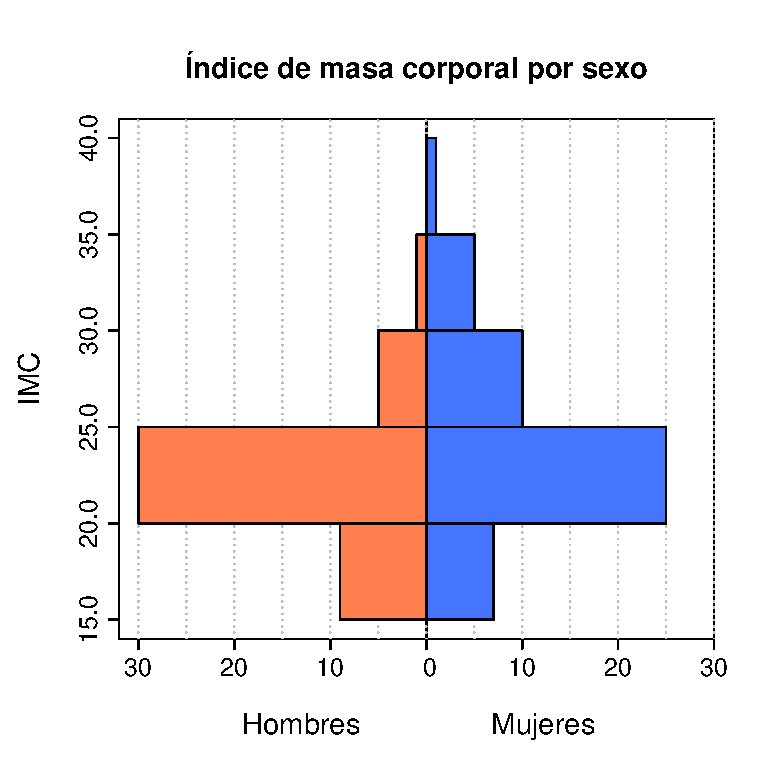
\includegraphics[scale=0.7]{img/histograma-des-29}
\end{center}
Se pide:
\begin{enumerate}
\item Construir la tabla de frecuencias para hombres y mujeres por separado.
\item Dibujar el diagrama de sectores para el sexo.
\item ¿En qué grupo es más representativa la media? Justificar la respuesta.
\item ¿Cómo calcularías la media de toda la muestra a partir de las medias de hombres y mujeres? ¿Cuánto vale?
\item Calcular el rango intercuartílico del índice de masa corporal en los hombres.
\end{enumerate}
}
%SOLUCIÓN
{\begin{enumerate}[start=3]
\item $\bar{m} =24.17$ Kg/m$^2$, $s_{m}^2=21.1806$ (Kg/m$^2$)$^2$, $s_m=4.6$ Kg/m$^2$ y $cv_m = 0.19$.\\
$\bar{h} =22.28$ Kg/m$^2$, $s_{m}^2=9.9506$ (Kg/m$^2$)$^2$, $s_m=3.15$ Kg/m$^2$ y $cv_h = 0.14$, luego es más representativa la media en los
hombres.
\item $\bar{x}=23.25$ Kg/m$^2$.
\item $RI=3.75$ Kg/m$^2$.
\end{enumerate}
}
%RESOLUCIÓN
{Lamemos $H$ a la variable que mide el índice de masa corporal para los hombres y $M$ para las mujeres.
\begin{enumerate}
\item A partir del histograma de frecuencias absolutas de las mujeres podemos obtener fácilmente las frecuencias absolutas de los intervalos mirando la altura de las barras, y a partir de las frecuencias absolutas podemos calcular el resto de frecuencias.
La tabla de frecuencias para las mujeres es:
\[
\begin{array}{|c|r|r|r|r|}
\hline
   M   & n_i &  f_i & N_i &  F_i \\
\hline
 15-20 &   7 & 0.15 &   7 & 0.15 \\
 20-25 &  25 & 0.52 &  32 & 0.67 \\
 25-30 &  10 & 0.21 &  42 & 0.88 \\
 30-35 &   5 & 0.10 &  47 & 0.98 \\
 35-40 &   1 & 0.02 &  48 & 1.00 \\
\hline
\mbox{Suma} & 48 & 1.00 & & \\
\hline
\end{array}
\]
Del mismo modo, a partir del histograma de frecuencias absolutas de los hombres obtenemos la tabla de frecuencias para hombres:
\[
\begin{array}{|c|r|r|r|r|}
\hline
   H   & n_i &  f_i & N_i &  F_i \\
\hline
 15-20 &   9 & 0.20 &   9 & 0.20 \\
 20-25 &  30 & 0.67 &  39 & 0.87 \\
 25-30 &   5 & 0.11 &  44 & 0.98 \\
 30-35 &   1 & 0.02 &  45 & 1.00 \\
\hline
\mbox{Suma} & 45 & 1.00 & & \\
\hline
\end{array}
\]

\item La variable Sexo sólo tiene dos categorías que son Hombre y Mujer, de modo que el diagrama de sectores asociado sólo tendrá dos sectores. La tabla de frecuencias de la variable sexo es:
\[
\begin{array}{|c|r|r|}
\hline
  \textrm{Sexo}  & n_i &   f_i \\
\hline
 \textrm{Mujer}  &  48 & 0.516 \\
\hline
 \textrm{Hombre} &  45 & 0.484 \\
\hline
  \textrm{Suma}  &  93 & 1.000 \\
\hline
\end{array}
\]
Así pues, para calcular el ángulo correspondiente a cada sector basta con multiplicar $360^{\circ}$ (el ángulo de la circunferencia completa) por la frecuencia relativa de cada categoría:
\[
\alpha_m=360^{\circ}0.516=186^{\circ}\qquad \alpha_h=360^{\circ}0.484=174^{\circ}.
\]
Y el diagrama de sectores asociados es:
\begin{center}
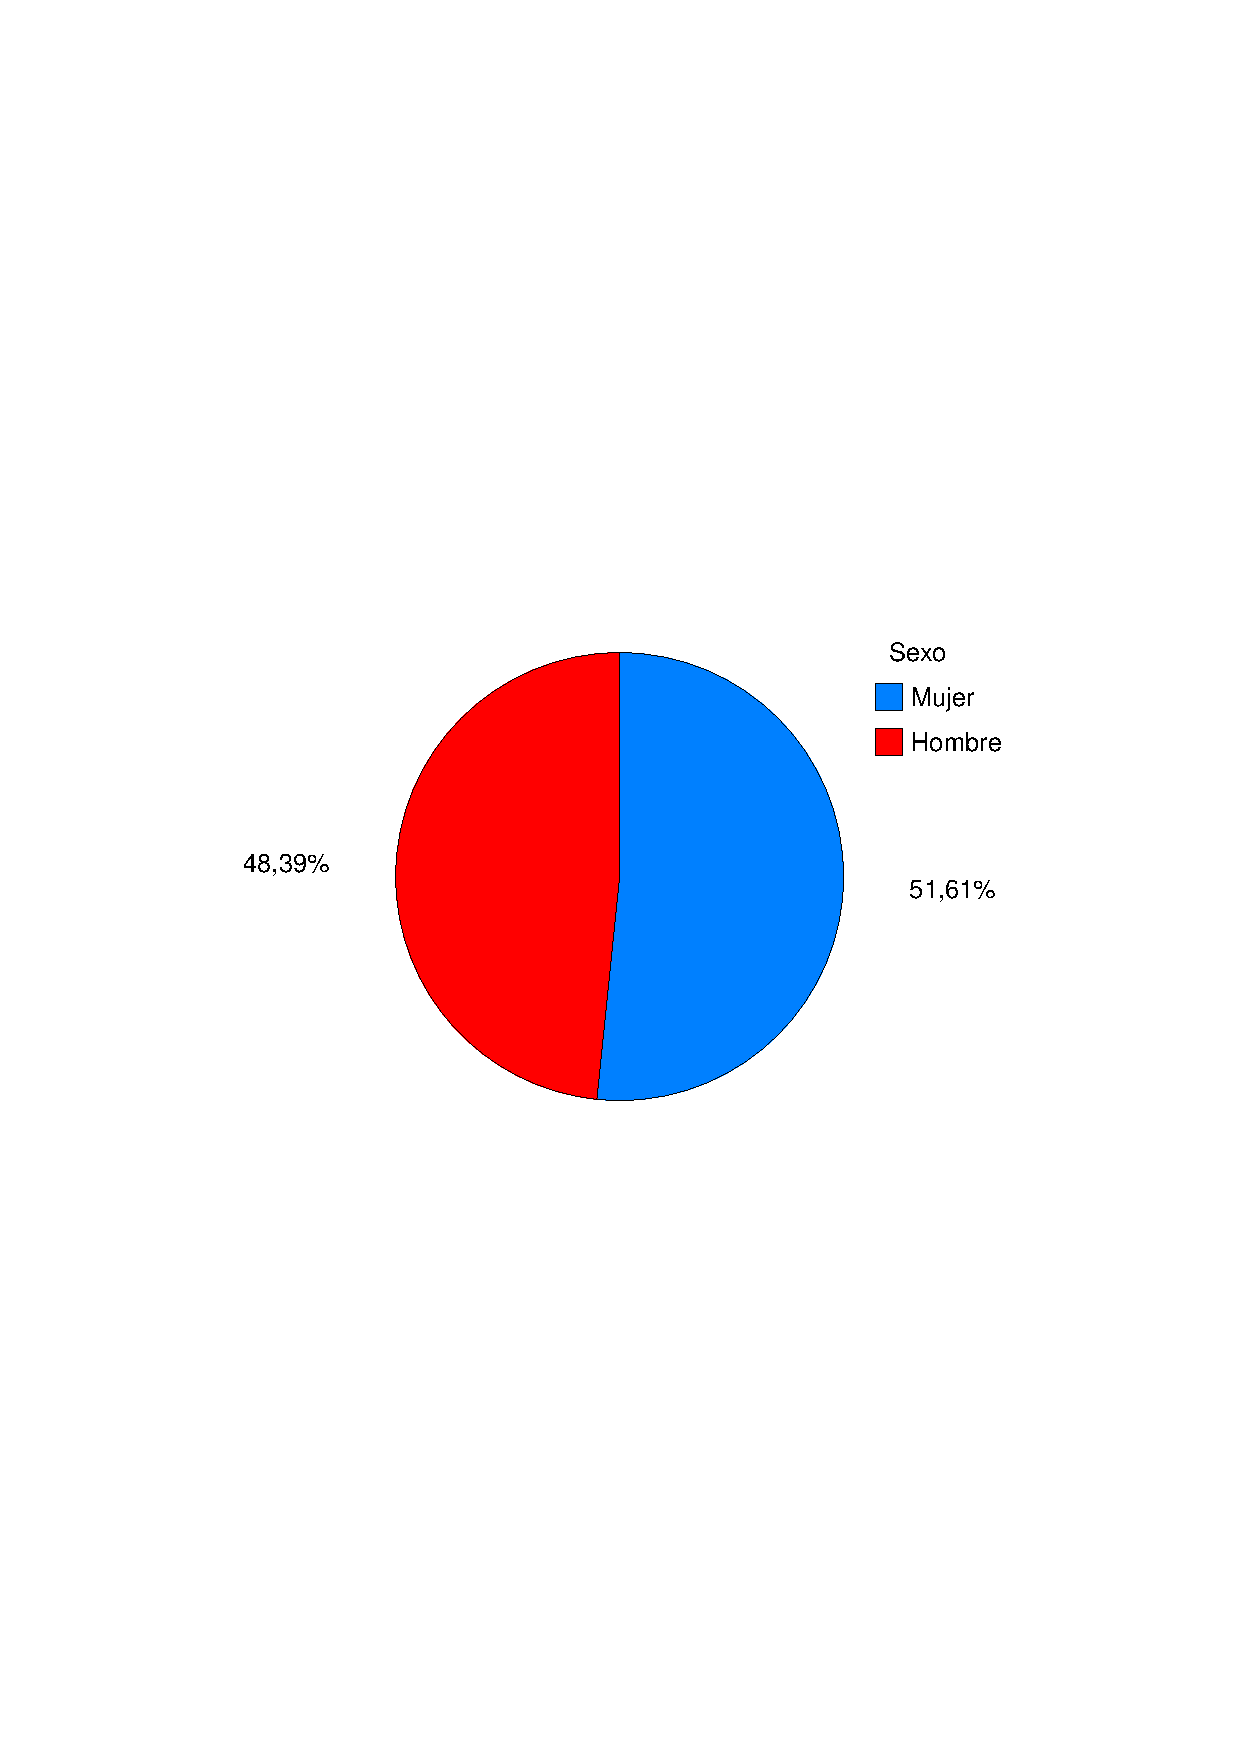
\includegraphics[scale=0.6]{img/sectores-des-29}
\end{center}

\item La media será más representativa en el grupo que tenga menos dispersión, y para comparar la dispersión de ambos grupos necesitamos el coeficiente de variación.
Calculamos para ello los estadísticos necesarios a partir de las tablas de frecuencias. Para las mujeres tenemos:
\[
\begin{array}{|c|r|r|r|r|}
\hline
   M   & m_i & n_i & m_in_i & m_i^2n_i \\
\hline
 15-20 & 17.5 &  7 & 122.5 & 2143.75 \\
 20-25 & 22.5 & 25 & 562.5 & 12656.25\\
 25-30 & 27.5 & 10 & 275.0 & 7562.50 \\
 30-35 & 32.5 &  5 & 162.5 & 5281.25 \\
 35-40 & 37.5 &  1 &  37.5 & 1406.25 \\
\hline
\mbox{Suma} & & 48 & 1160.0& 29050.00 \\
\hline
\end{array}
\]

\begin{align*}
\bar{m} & = \frac{\sum m_{i}}{n_m}=\frac{1160}{48}=24.17,  \\
s_{m}^2 &= \frac{\sum m_{i}^2}{n_m}-\bar{m}^2 = \frac{29050}{48}-24.17^2=21.1806,  \\
s_m &= \sqrt{21.1806} = 4.6,\\
cv_m &= \frac{s_m}{|\bar{m}|}=\frac{4.6}{24.17} = 0.19.
\end{align*}

Y para los hombres:
\[
\begin{array}{|c|r|r|r|r|}
\hline
   H   & h_i &  n_i & h_in_i &  h_i^2n_i \\
\hline
 15-20 &  17.5 &  9 & 157.5 &  2756.25 \\
 20-25 &  22.5 & 30 & 675.0 & 15187.50 \\
 25-30 &  27.5 &  5 & 137.5 &  3781.25 \\
 30-35 &  32.5 &  1 &  32.5 &  1056.25 \\
\hline
\mbox{Suma} & & 45 & 1002.5 & 22781.25 \\
\hline
\end{array}
\]

\begin{align*}
\bar{h} & = \frac{\sum h_{i}}{n_h}=\frac{1002.5}{45}=22.28,  \\
s_{h}^2 & = \frac{\sum h_{i}^2}{n_h}-\bar{h}^2 =
\frac{22781.25}{45}-22.28^2=9.9506,  \\
s_h &= \sqrt{9.9506} = 3.15,\\
cv_h &= \frac{s_h}{|\bar{h}|}=\frac{3.15}{22.28} = 0.14.
\end{align*}

Así pues, ambas muestras tienen un coeficiente de variación bajo y por tanto las medias son muy representativas, pero lo es un poco más la de los hombres ya que tienen una poca menos dispersión.

\item Para calcular la media de toda la muestra podemos hacer una media ponderada de las medias de las mujeres y l
os hombres donde los pesos son los tamaños muestrales de cada grupo.
\[
\bar{x}=\frac{p_m\bar{m}+p_h\bar{h}}{p_m+p_h}=\frac{45\cdot 22.28+48\cdot 24.17}{45+48}=23.25.
\]

\item El rango intercuartílico es la diferencia entre el tercer y el primer cuartil, así que procedemos a calcular ambos cuartiles.
La frecuencia acumulada correspondiente al primer cuartil es $n_h/4=11.25$, lo cual nos indica, mirando la columna de frecuencia acumuladas de los hombres, que dicho cuartil está en el intervalo $20-25$.
Interpolando en dicho intervalo tenemos:
\[C_1=20+\frac{11.25-9}{30}5 = 20.375.\]
Del mismo modo, la frecuencia acumulada correspondiente al tercer cuartil es $3n_h/4=33.75$, lo que indica que este cuartil también está en el intervalo $20-25$.
Interpolando en dicho intervalo tenemos:
\[C_3=20+\frac{33.75-9}{30}5 = 24.125.\]
Así pues, el rango intercuartílico es $RI=C_3-C_1=24.125-20.375=3.75$.
\end{enumerate}
}


\newproblem*{des-30}{med}{*}
%ENUNCIADO
{Se ha medido el tiempo necesario, en días, para curar un tipo concreto de infección (tiempo transcurrido desde el comienzo del tratamiento hasta el alta) en dos grupos de pacientes a los que se han aplicado antibióticos diferentes.
En un grupo de 80 pacientes tratados con el antibiótico A, los resultados obtenidos fueron:
\[
\begin{array}{|c|c|}
\hline
\mbox{Tiempo (días)} & n_i \\
\hline
{[0,30)} & 50 \\
{[30,60)} & 20 \\
{[60,90)} & 10 \\
\hline
\end{array}
\]

Mientras que en un grupo de 100 pacientes tratados con el antibiótico B se obtuvo:
\[
\begin{array}{|c|c|}
\hline
\mbox{Tiempo (días)} & n_i \\
\hline
{[0,30)} & 40 \\
{[30,60)} & 50 \\
{[60,90)} & 10 \\
\hline
\end{array}
\]

\begin{enumerate}
\item Calcular la media y la desviación típica del número de días hasta el alta, para cada uno de los antibióticos.
\item ¿En qué antibiótico es más representativa la media?. Justificar la respuesta numéricamente.
\item ¿Cuánto vale el percentil 90 del tiempo de curación para los pacientes tratados con B?
\item ¿Qué tiempo de recuperación ha sido relativamente más alto, uno de 40 días de un paciente tratado con A, o uno de 45 días de otro tratado con B? Justificar la respuesta numéricamente.
\end{enumerate}
}


\newproblem{des-31}{med}{*}
%ENUNCIADO
{Para  estudiar la eficacia de un nuevo fármaco en el tratamiento de la hipertensión arterial, se tomaron los valores
de la tensión arterial diastólica (TAD) en 8 pacientes antes del tratamiento ($X$) y después de un mes de tratamiento
($Y$), obteniéndose los siguientes resultados:
\begin{center}
\begin{tabular}{|c|r|r|r|r|r|r|r|r|}
\hline
$X$ & 100 & 104 & 96 & 98 & 105 & 106 & 110 & 100 \\
\hline
$Y$ & 92 & 97 & 94 & 100 & 94 & 92 & 95 & 104 \\
\hline
\end{tabular}
\end{center}

\begin{enumerate}
\item ¿En qué variable es más representativa la media?
\item Hallar el coeficiente de asimetría de la variable $Y$ e interpretarlo.
\end{enumerate}
}
%SOLUCIÓN
{\begin{enumerate}
\item $\bar x=102.375$, $s_x^2=18.9844$, $s_x=4.3571$ y $cv_x =0.0426$.\\
$\bar y=96$, $s_y^2=15.25$, $s_y=3.9051$ y $cv_y = 0.0407$.\\
Como ambos coeficientes de variación son casi iguales podemos concluir que ambas medias son igual de representativas.
\item $g_1=0.9068$ lo que indica que es asimétrica hacia la derecha.
\end{enumerate}
}
%RESOLUCIÓN
{\begin{enumerate}
\item Para ver en qué muestra es más representativa la media tenemos que comparar las dispersiones de ambas muestras mediante el coeficiente de variación. Para ello, procedemos al cálculo de los estadísticos necesarios:
\begin{align*}
\bar{x} & = \frac{\sum x_{i}}{n}=\frac{100+\cdots+100}{8}=\frac{819}{8}=102.375,  \\
s_{x}^2 & = \frac{\sum x_{i}^2}{n}-\bar{x}^2 =
\frac{100^2+\cdots+100^2}{8}-102.375^2=\frac{83997}{8}-10480,6406=18.9844,  \\
s_{x} & = \sqrt{18.9844}=4.3571,  \\
cv_x &= \frac{s_x}{|\bar{x}|}= \frac{4.3571}{102.375}=0.0426,\\
\bar{y} & = \frac{\sum y_{j}}{n}=\frac{92+\cdots+104}{8}=
\frac{768}{8}=96,  \\
s_{y}^2 & = \frac{\sum y_{j}^2}{n}-\bar{y}^2 =
\frac{92^2+\cdots+104^2}{8}-96^2=\frac{73850}{8}-9216=15.25,  \\
s_{y} & = \sqrt{15.25}=3.9051,  \\
cv_y &= \frac{s_y}{|\bar{y}|}= \frac{3.9051}{96}=0.0407,\\
\end{align*}
Ambos coeficientes de variación son muy pequeños, lo cual indica que hay muy poca dispersión en las muestras y las medias son muy representativas, aunque un poco más la de $Y$ por tener un coeficiente de variación más pequeño.

\item El coeficiente de asimetría de $Y$ es 
\[g_1=\frac{\sum(y_j-\bar{y})^3/n}{s_y^3}=
\frac{\left((92-96)^3+\cdots +(104-96)^3\right)/8}{3.9051^3}=\frac{432/8}{59,552}=0.9068,\]
lo que indica que la distribución es asimétrica a la derecha aunque no los suficiente como para rechazar la hipótesis de que los datos provienen de una población normal.
\end{enumerate}
}


\newproblem{des-32}{amb}{*}
%ENUNCIADO
{Una piscifactoría realiza un estudio para determinar si una especie de pez está en peligro extinción en los ríos de una región.
Para ello se midió el número de peces en 10 sitios diferentes obteniendo los siguientes resultados en unidades
por hectómetro cúbico:
\begin{center}
  36 -- 11 -- 7 -- 18 -- 35 -- 27 -- 21 -- 15 -- 25 -- 12
\end{center}
Se pide:
\begin{enumerate}
\item Calcular las medidas de tendencia central.
\item Calcular el coeficiente de apuntamiento e interpretarlo.
\end{enumerate}
}
%SOLUCIÓN
{\begin{enumerate}
\item $\bar{x} = 20.7$ peces, $Me=19.5$ peces, no hay moda porque todos los valores tienen frecuencia 1. 
\item $g_2= -1.13$ lo que indica que es una distribución bastante platicúrtica. 
\end{enumerate}
}
%RESOLUCIÓN
{Llamemos $X$ al número de peces por hectómetro cúbico.
\begin{enumerate}
\item Las medidas de tendencia central son la media aritmética, la mediana y la moda. Calculamos primero la media:
\[
\bar{x} = \frac{\sum x_{i}}{n}=\frac{36+\cdots+12}{10}=\frac{207}{10}=20.7 \mbox{ peces},
\]

Para calcular la mediana ordenamos los valores de la muestra:
\begin{center}
  7 -- 11 -- 12 -- 15 -- 18 -- 21 -- 25 -- 27 -- 35 -- 36
\end{center}
Como el tamaño de la muestra es par, habrá dos individuos que ocupen las posiciones centrales de la muestra, y estos serán los que ocupen las posiciones $n/2=10/2=5$ y $n/2+1=6$, es decir, los valores 18 y 21. Así pues la mediana es
\[
Me=\frac{18+21}{2}=19.5 \mbox{ peces}.
\]

Por último, no podemos decir que haya moda porque todos los valores tienen frecuencia 1.

\item La fórmula del coeficiente de apuntamiento es 
\[
g_2=\frac{\sum (x_i-\bar{x})^4}{ns^4}-3,
\]
así que necesitamos calcular previamente la desviación típica:
\begin{align*}
s^2 & = \frac{\sum x_{i}^2}{n}-\bar{x}^2 =
\frac{36^2+\cdots+12^2}{10}-20.7^2=\frac{5179}{10}-428,49=89.41,\\
s &=\sqrt{89.41}=9.4557.
\end{align*}
Así pues, tenemos
\[
g_2=\frac{(36-20.7)^4+\cdots + (12-20.7)^4}{10\cdot 9.4557^4}-3=\frac{149449.657}{79941,9504}-3=-1.13,
\]
lo que indica que la distribución es bastante platicúrtica, es decir, con menos apuntamiento que una distribución normal.
\end{enumerate}
}


\newproblem{des-33}{amb}{*}
%ENUNCIADO
{Las temperaturas (en ºC) observadas en Barcelona y La Coruña en 12 días elegidos aleatoriamente el último año fueron:
\begin{center}
\begin{tabular}{|l|cccccccccccc|}
\hline
Barcelona & 13 & 14 & 16 & 18 & 21 & 25 & 28 & 28 & 25 & 21 & 17 & 13\\ \hline
La Coruña & 13 & 13 & 15 & 16 & 17 & 20 & 22 & 23 & 22 & 19 & 15 & 13\\ \hline
\end{tabular}
\end{center}
Se pide:

\begin{enumerate}
\item ¿En cuál de las dos ciudades hay mayor variación de temperaturas?
\item ¿Por debajo de qué valor estarán las temperaturas de la mitad de los días en ambas ciudades?
\end{enumerate}
}
%SOLUCIÓN
{\begin{enumerate}
\item $cv_b = 0.2684$ y $cv_c =0.2071$ lo que indica que hay una ligera mayor variación de temperaturas en Barcelona.
\item $Me_b = 19,5.$ y $Me_c= 16.5$.
\end{enumerate}
}
%RESOLUCIÓN
{Llamemos $B$ a la variable que mide las temperaturas en Barcelona, y $C$ a la que mide las temperaturas en La Coruña.
\begin{enumerate}
\item Para ver en qué ciudad hay mayor variación de temperatura tenemos que calcular los coeficientes de variación de ambas ciudades y compararlos.
\begin{align*}
\bar{b} &=\frac{\sum b_i}{n}= \frac{13+14+\cdots+13}{12}=\frac{239}{12}=19.9167,\\
s_b^2 &= \frac{\sum b_i^2}{n}-\bar{b}^2=\frac{13^2+14^2+\cdots+13^2}{12}-19.9167^2=\frac{5103}{12}-396.6749=28.5764,\\
s_b &=\sqrt{28.5764}=5.3457,\\
cv_b &= \frac{s_b}{|\bar{b}|}=\frac{5.3457}{19.9167}=0.2684,\\
\bar{c} &=\frac{\sum c_i}{n}= \frac{13+13+\cdots+13}{12}=\frac{208}{12}=17.3333,\\
s_c^2 &= \frac{\sum c_i^2}{n}-\bar{c}^2=\frac{13^2+13^2+\cdots+13^2}{12}-17.3333^2=\frac{3760}{12}-300.4433=12.8889,\\
s_c &=\sqrt{12.8889}=3.5901,\\
cv_c &= \frac{s_c}{|\bar{c}|}=\frac{3.5901}{17.3333}=0.2071.
\end{align*}
Por consiguiente, como el coeficiente de variación es mayor en Barcelona, es en esta ciudad donde hay mayor variación de temperaturas.

\item El valor que cumple que por debajo del mismo están la mitad de los valores de la muestra es la mediana.
Para calcular la mediana en ambas ciudades ordenamos los valores de la muestra de menor a mayor, y puesto que tenemos un tamaño muestral par $n=12$, buscamos los dos valores centrales, que ocuparan las posiciones $n/2=6$ y $n/2+1=7$.
En el caso de Barcelona tenemos que dichos valores son
\begin{center}
\begin{tabular}{|c|cccccccccccc|}
\hline
Posición & 1 & 2 & 3 & 4 & 5 & 6 & 7 & 8 & 9 & 10 & 11 & 12   \\ \hline
B & 13 & 13 & 14 & 16 & 17 & \fbox{18} & \fbox{21} & 21 & 25 & 25 & 28 & 28 \\ \hline
\end{tabular}
\end{center}
Como son valores diferentes, la mediana es $Me_b=\dfrac{18+21}{2}=19,5.$

En el caso de La Coruña tenemos
\begin{center}
\begin{tabular}{|c|cccccccccccc|}
\hline
Posición & 1 & 2 & 3 & 4 & 5 & 6 & 7 & 8 & 9 & 10 & 11 & 12   \\ \hline
C & 13 & 13 & 13 &  15 & 15 & \fbox{16} & \fbox{17} & 19 & 20 & 22 & 22 & 23 \\ \hline
\end{tabular}
\end{center}
Y al igual que antes, la mediana es $Me_c=\dfrac{16+17}{2}=16,5.$
\end{enumerate}
}


\newproblem{des-34}{gen}{*}
%ENUNCIADO
{Las pruebas de determinación del cociente intelectual realizadas en un colectivo de alumnos universitarios
reflejan los siguientes resultados:
\begin{center}
\begin{tabular}{|c|c|}
\hline
   C.I.    & Nº de alumnos \\
\hline
  [80,90)  &       3       \\
\hline
 [90,100)  &      12       \\
\hline
 [100,110) &      21       \\
\hline
 [110,120) &      24       \\
\hline
 [120,130) &      13       \\
\hline
 [130,140) &       2       \\
\hline
\end{tabular}
\end{center}
\begin{enumerate}
\item Calcular el coeficiente de variación del cociente intelectual. ¿Es representativa la media?
\item Si se considera ``muy inteligente'' a una persona cuyo cociente intelectual se encuentra en el 10\% de los más inteligentes, ¿cuál será el cociente que delimita la categoría ``muy inteligente'' en el colectivo de alumnos?
\end{enumerate}
}
%SOLUCIÓN 
{\begin{enumerate}
\item $cv=0.1$ lo que indica que hay poca dispersión y la media es muy representativa.
\item $P_{90}=125.77$.
\end{enumerate}
}
%RESOLUCIÓN
{\begin{enumerate}
\item Para calcular el coeficiente de variación necesitamos la media y la desviación típica.
Para facilitar los cálculos, añadimos dos nuevas columnas a la tabla de distribución de frecuencias:
\[
\begin{array}{|c|c|r|r|r|}
\hline
   \textrm{C.I.}   & x_i & \multicolumn{1}{c|}{n_i} & \multicolumn{1}{c|}{x_in_i} & \multicolumn{1}{c|}{x_i^2n_i}\\
\hline\hline
  [80,90)  &  85  &   3       & 255 & 21675 \\
\hline
 [90,100)  &  95 &    12       & 1140 & 108300 \\
\hline
 [100,110) &  105 &    21       & 2205 & 231525\\
\hline
 [110,120) &  115 &    24       & 2760 & 317400\\
\hline
 [120,130) &  125 &    13       & 1625 & 203125\\
\hline
 [130,140) &  135 &     2       & 270 & 36450\\
\hline\hline
 \textrm{Sumas} &  & 75 & 8255 & 918475 \\
\hline
\end{array}
\]
A partir de aquí calculamos los estadísticos que necesitamos.
\begin{align*}
\bar{x} & = \frac{\sum x_in_i}{N}=\frac{8255}{75}=110.07,\\
s^2 & =\frac{\sum x_i^2n_i}{N}-\bar{x}^2= \frac{918475}{75}-110.07^2=131.6622,\\
s & =\sqrt{131.6622}=11.47.
\end{align*}
Finalmente calculamos el coeficiente de variación:
\[
cv=\frac{s}{|\bar{x}|}=\frac{11.47}{110.07}= 0.1.
\]
Puesto que el coeficiente de variación es pequeño, podemos concluir que hay poca dispersión en la muestra y por tanto, la media es representativa.

\item Buscamos el coeficiente intelectual por encima del cual está el 10\% más inteligente de la clase, o lo que es lo mismo, por debajo del cual está el 90\% menos inteligente de la clase. En definitiva se trata de calcular el percentil 90. 
Para ello necesitamos la columna de frecuencias acumuladas en la tabla
\[
\begin{array}{|c|r|r|}
\hline
   \textrm{C.I.}    & \multicolumn{1}{c|}{n_i} & \multicolumn{1}{c|}{N_i} \\
\hline\hline
  [80,90)  &       3       & 3 \\
\hline
 [90,100)  &      12       & 15 \\
\hline
 [100,110) &      21       & 36 \\
\hline
 [110,120) &      24       & 60 \\
\hline
 [120,130) &      13       & 73 \\
\hline
 [130,140) &       2       & 75 \\
\hline
\end{array}
\]

La frecuencia acumulada correspondiente al percentil 90 es $N_{P_{90}}=90\cdot 75/100=67.5$. Mirando el la  columna de frecuencias acumuladas de la tabla de frecuencias comprobamos que dicha frecuencia se alcanza dentro del intervalo $[120,130)$.
Interpolando en este intervalo obtenemos el percentil que buscamos \[P_{90}=120+\frac{67.5-60}{13}10=125.77.\]
\end{enumerate}
}


\newproblem{des-35}{far}{*}
%ENUNCIADO
{En un laboratorio farmacéutico se van a fabricar dos tipos de cápsulas $A$ y $B$, cuyos contenidos en principio
activo debe ser 250 y 500 mg. respectivamente. Para ello se prueban dos máquinas dosificadoras, una para cada tipo de
cápsulas, siendo los contenidos en principio activo de las cápsulas fabricadas con ellas los siguientes:
\[
\begin{array}{c|c}
A & B  \\ \hline
238 & 488  \\
245 & 494  \\
236 & 476  \\
248 & 483  \\
241 & 492  \\
243 &
\end{array}
 \]
¿En cuál de las dos máquinas es más representativa la media?
Razonar la respuesta.
}
%SOLUCIÓN
{$cv_{A} = 0.0167$ y $cv_{B}=0.0133$, luego es un poco más representativa la media en la máquina $B$. 
}
%RESOLUCIÓN
{Llamaremos $A$ a la variable que mide la cantidad de principio activo que pone la máquina $A$ en cada cápsula y $B$ a la variable que mide la cantidad de principio activo que pone la máquina $B$ en cada cápsula.
Para ver en cual de las dos muestras es más representativa la media, tenemos que calcular los coeficientes de variación en cada caso. 

Calculamos primero los estadísticos necesarios para la máquina $A$:
\begin{align*}
\bar{A} & = \frac{\sum A_{i}}{n_{A}}=\frac{1451}{6}=241.833,\\
s_{A}^2 & =  \frac{\sum{A_{i}^2}{n_{A}}}-\bar{A}^2= \frac{350999}{6}-241.833^2=16.472,\\
s_{A} & = \sqrt{16.472}= 4.058,\\
cv_{A} & = \frac{s_{A}}{\bar{A}}=\frac{4.058}{241.833}=0.0167,
\end{align*}

En el caso de la máquina $B$ tenemos:
\begin{align*}
\bar{B} & = \frac{\sum B_{i}}{n_{B}}=\frac{2433}{5}=486.6,\\
s_{B}^2 & = \frac{\sum{B_{i}^2}{n_{B}}}-\bar{B}^2= \frac{1184109}{5}-486.6^2=42.24,\\
s_{B} & = \sqrt{42.24}= 6.499,\\
cv_{B} & = \frac{s_{B}}{\bar{B}}=\frac{6.499}{486.6}=0.0133.
\end{align*}

Como el coeficiente de variación de la muestra de $B$ es un poco menor que el de $A$, la dispersión será menor en la muestra de $B$ y $\bar{B}$ será un poco más representativa que $\bar{A}$.
}


\newproblem{des-36}{gen}{*}
%ENUNCIADO
{En un centro de reclutamiento se han medido las alturas de 150 jóvenes, obteniéndose la siguiente tabla de frecuencias:
\[
\begin{tabular}{|c|c|}
\hline
Altura: & Número de jóvenes: \\ \hline
1.50-1.60 & 12 \\ \hline
1.60-1.70 & 30 \\ \hline
1.70-1.80 & 52 \\ \hline
1.80-1.90 & 42 \\ \hline
1.90-2.00 & 11 \\ \hline
2.00-2.10 & 3 \\ \hline
\end{tabular}
\]

\begin{enumerate}
\item Calcular el coeficiente de variación. ¿Es representativa la media?
\item  Si se considera alto a un joven cuya altura corresponde como mínimo a la del percentil 85, ¿cuál es la
mínima altura que tendrá un alto?
\end{enumerate}
}
%SOLUCIÓN
{\begin{enumerate}
\item $cv=0.065$ lo que indica muy poca dispersión y una media muy representativa.
\item $ P_{85}=1.88$ mt.
\end{enumerate}
}
%RESOLUCIÓN
{\begin{enumerate}
\item  El coeficiente de variación se define como
\[
cv=\dfrac{s}{|\bar{x}|},
\]
de modo que necesitamos calcular la media y la desviación típica, pero antes de nada, completamos la tabla de frecuencias.
\[
\begin{array}{|c|c|c|c|c|}
\hline
x_{i} & n_{i} & N_{i} & x_{i}n_{i} & x_{i}^2n_{i}\\ \hline
1.50-1.60 & 12 & 12 & 18.6 & 28.83 \\
1.60-1.70 & 30 & 42 & 49.5 & 81.68 \\
1.70-1.80 & 52 & 94 & 91 & 159.25\\
1.80-1.90 & 42 & 136 & 77.7 & 143.75\\
1.90-2.00 & 11 & 147 & 21.45 & 41.83\\
2.00-2.10 & 3 & 150 & 6.15 & 12.61\\ \hline
\mbox{Sumas} & 150 & & 264.4 & 467.94 \\
\hline
\end{array}
\]
Ahora calculamos la media y la desviación típica:
\begin{eqnarray*}
\bar{x} & = & \frac{\sum
x_{i}n_{i}}{N}=\frac{264.4}{150}=1.7627.\\
s^2 & = & \frac{\sum x_{i}^2 n_{i}}{N}-\bar{x}^2 =
\frac{467.94}{150}-1.7627^2=0.013.\\
s & = & \sqrt{0.02}=0.114.
\end{eqnarray*}
Por consiguiente, el coeficiente de variación es
\[ cv=\frac{0.114}{1.7627}=0.065, \]
lo que indica que hay muy poca dispersión y la media es muy representativa.

\item Tenemos que calcular el percentil 85 para ver a partir de qué estatura un joven es considerado alto.
La frecuencia absoluta acumulada correspondiente al percentil 85 es $85\cdot N/100=85\cdot 150/100 = 127.5$. 
Mirando la tabla de frecuencias en la columna de las frecuencias absolutas acumuladas podemos comprobar que la frecuencia 127.5 se alcanza en algún punto del intervalo 1.80-1.90.
Para obtener el percentil 85 interpolamos en dicho intervalo:
\[ P_{85}=1.80+\frac{127.5-94}{42}(1.90-1.80)=1.88. \]
\end{enumerate}
}


\newproblem{des-37}{med}{*}
%ENUNCIADO
{Se ha realizado un estudio sobre la tensión arterial en dos ciudades A y B. Se tomó una muestra de 20 individuos, que arrojó los siguientes valores:
\begin{center}
\begin{tabular}{l}
\begin{tabular}{|l|c|c|c|c|c|c|c|c|c|c|}
\hline
 Tensión & 135 & 128 & 137 & 110 & 154 & 142 & 121 & 127 & 114 & 103 \\
\hline
 Ciudad  &  A  &  B  &  A  &  B  &  A  &  A  &  A  &  B  &  B  &  B  \\
\hline
\end{tabular}
\\[.5cm]
\begin{tabular}{|l|c|c|c|c|c|c|c|c|c|c|}
\hline
 Tensión & 98 & 96 & 114 & 123 & 132 & 141 & 132 & 121 & 98 & 136 \\
\hline
 Ciudad  & A  & B  &  A  &  B  &  A  &  B  &  A  &  B  & B  &  A  \\
\hline
\end{tabular}
\end{tabular}
\end{center}
Se pide:
\begin{enumerate}
\item Construir la tabla de frecuencias para la tensión, agrupando en clases de amplitud 10, entre 95 y 155.
\item Dibujar el polígono de frecuencias acumuladas correspondiente a la tabla anterior.
\item Calcular el coeficiente de asimetría e interpretarlo.
\item Calcular el tercer decil e interpretarlo.
\item Considerando los datos sin agrupar, ¿en qué ciudad son más homogéneas las tensiones?
\end{enumerate}
}
%SOLUCIÓN
{\begin{enumerate}[start=3]
\item $\bar x = 123$ mmHg, $s^2= 251$ mmHg$^2$, $s=15.843$ mmHg y $g_1=-0.12$, por lo que la distribución es un poco asimétrica hacia la izquierda.
\item $D_3= 111,67$ mmHg.
\item $\bar x_A=130.1$ mmHg, $s^2_A=219.89$ mmHg$^2$, $s_A=14.8287$ mmHg y $cv_A =0.1139$.\\
$\bar x_B=116.1$ mmHg, $s^2_B=189.69$ mmHg$^2$, $s_B=13.7728$ mmHg y y $cv_B = 0.1186$.
Así pues, como el $cv_A<cv_B$ las tensiones son un poco más homogéneas en la ciudad $A$, aunque en ambos casos las muestras son muy homogéneas. 
\end{enumerate}
}
%RESOLUCIÓN
{Llamemos $X$ a la variable que mide la tensión arterial.
\begin{enumerate}
\item Agrupando en clases de amplitud 10, obtenemos 6 clases entre 95 y 155. La tabla de frecuencias correspondiente es 
\[
\begin{array}{|c|r|r|r|r|r|}
\hline
   X  & \multicolumn{1}{c|}{x_i} & \multicolumn{1}{c|}{n_i} & \multicolumn{1}{c|}{f_i} & \multicolumn{1}{c|}{N_i} & \multicolumn{1}{c|}{F_i}\\
\hline\hline
  [95,105)  &  100  &   4       & 0.2 & 4 & 0.2\\
\hline
 [105,115)  &  110 &    3       & 0.15 & 7 & 0.35 \\
\hline
 [115,125) &  120 &    3       & 0.15 &  10 & 0.5\\
\hline
 [125,135) &  130 &    4       & 0.2 & 14 & 0.7\\
\hline
 [135,145) &  140 &    5       & 0.25 & 19 & 0.95\\
\hline
 [145,155) &  150 &     1       & 0.05 & 10 & 1\\
\hline
\end{array}
\]

\item El polígono de frecuencias absolutas acumuladas correspondiente a esta tabla es el siguiente
\begin{center}
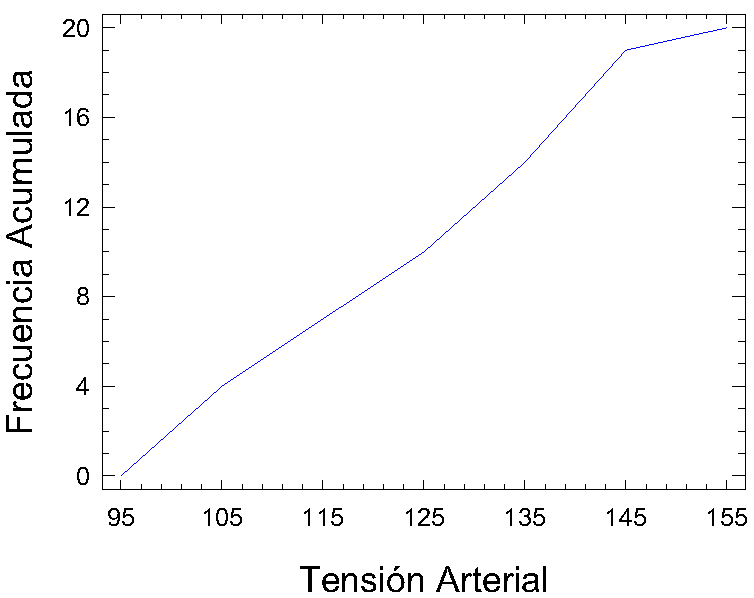
\includegraphics[scale=0.6]{img/poligono-tension-des-37}
\end{center}

\item El coeficiente de asimetría se calcula mediante la fórmula 
\[g_1=\frac{\sum (x-\bar{x})^3n_i/n}{s^3}.\]
A partir de la tabla anterior, calculamos los estadísticos necesarios: 
\[
\begin{array}{|c|r|r|r|r|}
\hline
   X  & \multicolumn{1}{c|}{x_i} & \multicolumn{1}{c|}{n_i} & \multicolumn{1}{c|}{x_in_i} & \multicolumn{1}{c|}{x_i^2n_i}\\
\hline\hline
  [95,105)  &  100  &   4       & 400 & 40000\\
\hline
 [105,115)  &  110 &    3       & 330 & 36300 \\
\hline
 [115,125) &  120 &    3       & 360 &  43200\\
\hline
 [125,135) &  130 &    4       & 520 & 67600 \\
\hline
 [135,145) &  140 &    5       & 700 & 98000 \\
\hline
 [145,155) &  150 &     1       & 150 & 22500\\
\hline
\hline
\textrm{Sumas} & & 20 & 2460 & 307600\\
\hline
\end{array}
\]

\begin{align*}
\bar{x} & = \frac{\sum x_in_i}{n}=\frac{2460}{20}=123,\\
s^2 & =\frac{\sum x_i^2n_i}{N}-\bar{x}^2= \frac{307600}{20}-123^2=251,\\
s & =\sqrt{251}=15.84.
\end{align*}

Por último calculamos el coeficiente de asimetría
\[
\begin{array}{|c|r|r|r|r|}
\hline
   X  & \multicolumn{1}{c|}{x_i} & \multicolumn{1}{c|}{n_i} & \multicolumn{1}{c|}{x_i-\bar{x}} & \multicolumn{1}{c|}{(x_i-\bar{x})^3n_i}\\
\hline\hline
  [95,105)  &  100  &   4       & -23 & -48668\\
\hline
 [105,115)  &  110 &    3       & -13 & -6591 \\
\hline
 [115,125) &  120 &    3       & -3 &  -81\\
\hline
 [125,135) &  130 &    4       & 7 & 1372 \\
\hline
 [135,145) &  140 &    5       & 17 & 24565 \\
\hline
 [145,155) &  150 &     1       & 27 & 19683\\
\hline
\hline
\textrm{Sumas} & & 20 &  & -9720\\
\hline
\end{array}
\]

\[
g_1=\frac{\sum (x-\bar{x})^3n_i/n}{s^3}=\frac{-9720/20}{15.84^3}=-0.12.
\]
Esto indica que la distribución es ligeramente asimétrica a la izquierda.

\item El tercer decil $D_3$ tiene frecuencia absoluta acumulada $N_{D_3}=3n/10=3\cdot 20/10=6$, y mirando en la columna de frecuencias absolutas acumuladas comprobamos que corresponderá a un individuo de la clase $[105,115)$. Interpolando en dicho intervalo tenemos que que el tercer decil es
\[ D_3=105+\frac{6-4}{3}10=111,67,
\]
lo cual indica que  el 30\% de la población tiene un tensión inferior a 111.67.

\item Llamemos $a$ y $b$ a las variables que miden las tensiones de las ciudades A y B respectivamente. Las tensiones serán más homogéneas en la ciudad que haya menos dispersión. Para comparar las dispersiones de ambas poblaciones utilizamos el coeficiente de variación que no depende de las unidades. Calculamos los estadísticos necesarios trabajando directamente desde la muestra sin agrupar:
\begin{align*}
\bar{a} & = \frac{\sum a_{i}}{n}=\frac{135+\cdots+136}{10}=\frac{1301}{10}=130.1,  \\
s_{a}^2 & = \frac{\sum a_{i}^2}{n}-\bar{a}^2 =
\frac{135^2+\cdots+136^2}{10}-130.1^2=\frac{171459}{10}-16926.01=219.89,  \\
s_{a} & = \sqrt{219.89}=14.83,  \\
cv_a &=\frac{s_a}{|\bar{a}|}=\frac{14.83}{130.1}=0.1139,\\
\bar{b} & = \frac{\sum b_{j}}{n}=\frac{128+\cdots+98}{10}=
\frac{1161}{10}=116.1,  \\
s_{b}^2 & = \frac{\sum b_{j}^2}{n}-\bar{b}^2 =
\frac{128^2+\cdots+98^2}{10}-116.1^2=\frac{136689}{10}-13479.21=189.69,  \\
s_{b} & = \sqrt{189.69}=13.77,  \\
cv_b &=\frac{s_b}{|\bar{b}|}=\frac{13.77}{116.1}=0.1186.
\end{align*}
Así pues, comparando los coeficientes de variación en ambas ciudades comprobamos que son prácticamente iguales aunque es un poco menor la dispersión en la ciudad A por lo que las tensiones serán un poco más homogéneas.
\end{enumerate}
}


\newproblem{des-38}{gen}{*}
%ENUNCIADO
{En un grupo de alumnos se ha medido el número de días que faltaron a clase una muestra de alumnos de primer año y otra de alumnos repetidores, obteniendo:
\[
\begin{array}{lcccccccc}
\mbox{Primer año:}  & 8 & 2 & 3  & 2  & 1  & 4 & 0 & 3 \\
\mbox{Repetidores:} & 4 & 6 & 20 & 12 & 16 & 8 & 5 &   \\
\end{array}
\]
Se pide:
\begin{enumerate}
\item Calcular la mediana en ambos casos.
\item ¿En cuál de las dos muestras hay menos dispersión?
\item ¿Comparar el apuntamiento de ambas muestras?
\end{enumerate}
}
%SOLUCIÓN
{\begin{enumerate}
\item $Me_{x}=2.5$ y $Me_{y}=8$.
\item $cv_x =0.7862$ y $cv_y =0.5538$, hay menos dispersión en los alumnos repetidores. 
\item $g_{2_x} =0.703$ y $g_{2_y} =-1.125$ lo que indica que la distribución de los alumnos de primer año es leptocúrtica y la de los repetidores platicúrtica.
\end{enumerate}
}
%RESOLUCIÓN
{Llamemos $X$ a la variable que mide el número de días que faltaron los alumnos de primer año, e $Y$ al de los alumnos repetidores
\begin{enumerate}
\item Para calcular la mediana primero ordenamos los datos de ambas muestras:
\[
\begin{array}{lcccccccc}
\mbox{Primer año:}  & 0 & 1 & 2  & 2  & 3  & 3 & 4 & 8 \\
\mbox{Repetidores:} & 4 & 5 & 6 & 8 & 12 & 16 & 20 &   \\
\end{array}
\]
En el primer caso, como el tamaño de la muestra es par, habrá dos valores que estarán en el centro de la distribución, que serán los que ocupen la posiciones $n/2=8/2=4$ y $n/2+1=5$, es decir, los valores 2 y 3, de modo que la mediana es su media:
\[
Me_{x}=\frac{2+3}{2}=2.5.
\]
En el segundo caso, como el tamaño muestral es impar, sólo habrá un valor central que será el que ocupe la posición $(n+1)/2=8/2=4$, es decir, el valor 8, y por tanto $Me_{y}=8$.

\item Para compara la dispersión de ambas muestras tenemos que calcular el coeficiente de variación, y para ello, previamente hay que calcular la media y la desviación típica de cada muestra:
\begin{align*}
\bar{x} & = \frac{\sum x_{i}}{n}=\frac{8+\cdots+3}{8}=\frac{23}{8}=2.875,  \\
s_{x}^2 & = \frac{\sum x_{i}^2}{n}-\bar{x}^2 =
\frac{8^2+\cdots+3^2}{8}-2.875^2=\frac{107}{8}-8,2656=5.1094,  \\
s_{x} & = \sqrt{5.1094}=2.2604,  \\
cv_x &=\frac{s_x}{|\bar{x}|}=\frac{2.2604}{2.875}=0.7862,\\
\bar{y} & = \frac{\sum y_{j}}{n}=\frac{4+\cdots+5}{7}=
\frac{71}{7}=10.143,  \\
s_{y}^2 & = \frac{\sum y_{j}^2}{n}-\bar{y}^2 =
\frac{4^2+\cdots+5^2}{7}-10.143^2=\frac{941}{7}-102.8804=31.5510,  \\
s_{y} & = \sqrt{31.5510}=5.617,  \\
cv_y &=\frac{s_y}{|\bar{y}|}=\frac{5.617}{10.143}=0.5538.
\end{align*}
Así pues, como el coeficiente de variación es menor en $Y$, hay menos dispersión el grupo de los repetidores.

\item El coeficiente de apuntamiento en ambas muestras es
\begin{align*}
g_{2_x} &=\frac{\sum (x_i-\bar{x})^4}{ns_x^4}-3= \frac{(8-2.875)^4+\cdots + (3-2.875)^4}{8\cdot 2.2604^4}-3=\frac{773.3379}{208.8484}-3=0.703,\\
g_{2_y} &=\frac{\sum (y_j-\bar{y})^4}{ns_y^4}-3= \frac{(4-10.143)^4+\cdots + (5-10.143)^4}{7\cdot 5.617^4}-3=\frac{13068.6239}{6968.1218}-3=-1.125.
\end{align*}
Por tanto, la primera muestra tiene un apuntamiento mayor de lo normal (leptocúrtica) mientras que la segunda muestra tiene un apuntamiento bastante menor de lo normal (platicúrtica). 
\end{enumerate}
}


\newproblem*{des-39}{nut}{*}
%ENUNCIADO
{Al realizar un estudio sobre el peso de las mujeres mayores de 30 años en una determinada población, se obtuvieron los siguientes datos:
\begin{center}
72 -- 66 -- 51 -- 87 -- 65 -- 57 -- 73 -- 84 -- 67 -- 78 \\
58 -- 62 -- 75 -- 56 -- 68 -- 74 -- 57 -- 65 -- 73 -- 67
\end{center}
Realizar un estudio descriptivo agrupando los datos en 4 clases de amplitud 10 comenzando en el 50, que incluya:
\begin{enumerate}
\item Histograma de frecuencias absolutas y frecuencias absolutas acumuladas y los correspondientes polígonos.
\item Rango intercuartílico e interpretación.
\item Estudiar la representatividad de la media.
\end{enumerate}
}


\newproblem*{des-40}{nut}{*}
%ENUNCIADO
{Se realiza un estudio sobre el nivel de colesterol en sangre de los trabajadores de una empresa que utilizan habitualmente el comedor de la misma. Los resultados fueron los siguientes:
\begin{center}
214 - 205 - 197 - 204 - 186 - 192 - 216 - 176 - 192 - 196\\
207 - 182 - 218 - 203 - 194 - 176 - 203 - 214 - 188 - 198 
\end{center}
Se pide:

\begin{enumerate}
\item Obtener la distribución de frecuencias agrupadas en clases de amplitud 10, comenzando en 170.
\item Dibujar el histograma y el polígono de frecuencias.
\item Calcular el coeficiente de variación de Pearson e interpretar los resultados.
\item Calcular el rango intercuartílico.
\end{enumerate}
}


\newproblem{des-41}{psi}{}
%ENUNCIADO
{En un grupo de alumnos universitarios se realiza un estudio sobre la velocidad de lectura.
Para ellos se les dio a leer un texto de un periódico y se contó el número de palabras que leyeron en un minuto, obteniendo los siguientes resultados:
\begin{center}
286 -- 242 -- 185 -- 244 -- 296 -- 211 -- 233 -- 179 -- 190 -- 274 \\
255 -- 222 -- 260 -- 216 -- 204 -- 247 -- 232 -- 257 -- 196 -- 261
\end{center}
Se pide:
\begin{enumerate}
\item Construir la tabla de frecuencias agrupando en intervalos de amplitud 25 comenzando en 175.
\item Calcular las medidas de tendencia central. ¿Es representativa la media?
\item Calcular el coeficiente de apuntamiento e interpretarlo.
\end{enumerate}
}
%SOLUCIÓN
{\begin{enumerate}[start=2]
\item $\bar{x}=233.75$, $Med=235$, $Mod= [225,250)$ y $[250-275]$. $s^2=1017.19$, $s=31.89$ y $cv=0.14$ lo que indica que hay poca dispersión y la media es muy representativa.
\item $g_2=-1.1$ de manera que la distribución es bastante platicúrtica. 
\end{enumerate}
}
%RESOLUCIÓN
{}


\newproblem*{des-42}{amb}{*}
%ENUNCIADO
{Una piscifactoría realiza un estudio para determinar si una especie de pez está en peligro extinción en los ríos de una región.
Para ello se midió el número de peces en 12 sitios diferentes obteniendo los siguientes resultados en unidades por hectómetro cúbico:
\begin{center}
  16 -- 11 -- 14 -- 18 -- 21 -- 27 -- 21 -- 15 -- 22 -- 12 -- 2 -- 19
\end{center}
Se pide:
\begin{enumerate}
\item Dibujar el diagrama de cajas y eliminar de la muestra los datos atípicos si existen.
\item Calcular las medidas de tendencia central. ¿Cuál de ellas es más representativa?
\item Calcular el coeficiente de apuntamiento e interpretarlo.
\end{enumerate}
}


\newproblem*{des-43}{gen}{*}
%ENUNCIADO
{Dado el siguiente polígono correspondiente a una muestra de 60 individuos
\begin{center}
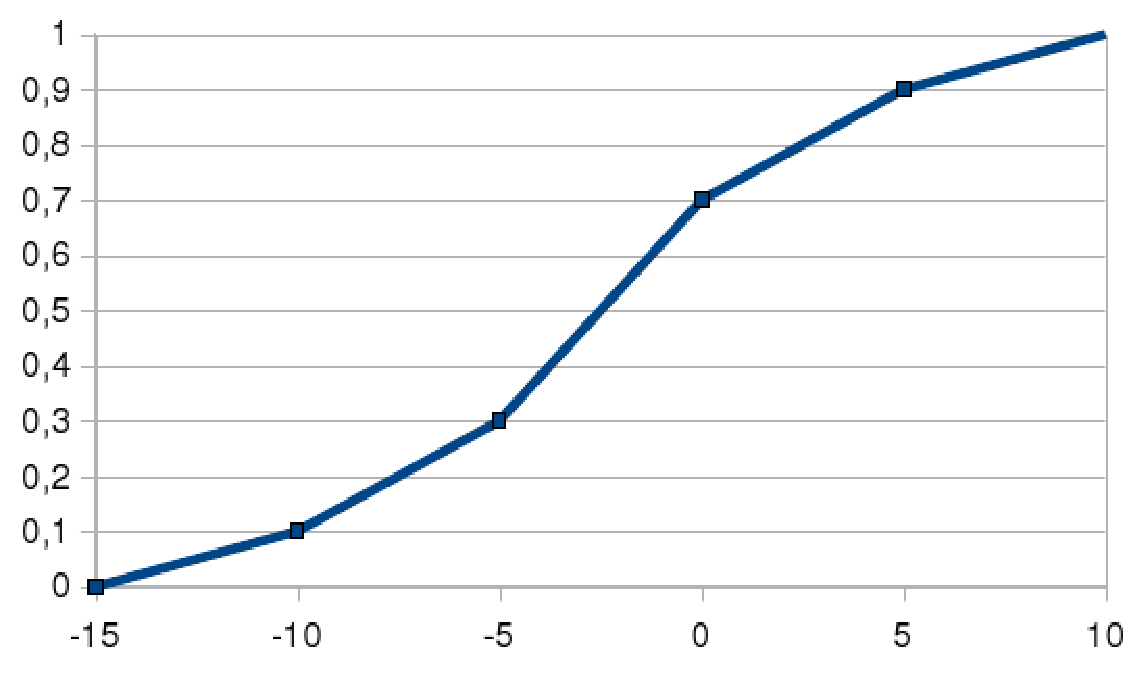
\includegraphics[scale=0.5]{img/poligono-acumuladas-des-43}
\end{center}
Calcular:
\begin{enumerate}
\item Tabla de frecuencias
\item Coeficiente de variación. ¿Se puede decir que hay mucha dispersión?
\item Decil 7.
\item Coeficiente de asimetría e interpretarlo.
\end{enumerate}
}


\newproblem*{des-44}{amb}{*}
%ENUNCIADO
{La siguiente tabla muestra los datos de emisiones de CO$_2$ y CH$_4$ (en Kg/hab) y el producto interior bruto per cápita (en miles US\$) de varios países en el último año:
\[
\begin{array}{|l|r|r|r|}
\hline
\mbox{País} & \mbox{CO}_2 & \mbox{CH}_4 & \mbox{PIB}\\
\hline\hline
\mbox{Austria}     & 7.60 & 0.97 & 38.40\\ \hline
\mbox{España}      & 6.73 & 0.81	& 30.12\\ \hline
\mbox{Francia}     & 5.71 & 0.94	& 33.19\\ \hline
\mbox{EEUU}        &19.40 & 1.72	&	45.84\\ \hline
\mbox{Alemania}    & 9.80 & 0.83	& 34.18\\ \hline
\mbox{Canadá}      &15.60 & 3.08	& 38.43\\ \hline
\mbox{Italia}      & 7.29 & 0.58	& 30.44\\ \hline
\mbox{Japón}       &	9.44 & 0.16	& 33.58\\ \hline
\mbox{Australia}   &17.48 & 6.36	& 36.26\\ \hline
\mbox{Reino Unido} & 8.99 & 0.76	& 35.13\\ \hline
\end{array}
\qquad
\begin{array}{|l|r|r|r|}
\hline
\mbox{País} & \mbox{CO}_2 & \mbox{CH}_4 & \mbox{PIB}\\
\hline\hline
\mbox{Bolivia}     & 1.05 & 3.44	& 40.13\\ \hline
\mbox{Niger}       &	0.1	 & 0.12	&	 0.67\\ \hline
\mbox{Senegal}     &	0.35 & 0.76 &  1.69\\ \hline
\mbox{Pakistán}    & 0.65 & 0.59	&  2.59\\ \hline
\mbox{Filipinas}   &	0.83 & 0.46	&  3.38\\ \hline
\mbox{Perú}        & 0.94 & 0.75	&  7.80\\ \hline
\mbox{Túnez}      & 2.17 & 0.48	&  7.47\\ \hline
\mbox{Nepal}       & 0.13 & 0.90	&  1.21\\ \hline
\mbox{Nicaragua}   & 0.7	 & 0.32	&  2.62\\ \hline
\mbox{Mauritania}  & 0.97 & 0.85	&  2.01\\ \hline
\end{array}
\]
Se pide:
Agrupar los datos de CH$_4$ en 5 clases desde el 0 hasta el 2 y calcular:
\begin{enumerate}
\item Media, varianza y coeficiente de variación. ¿Existe mucha dispersión? Justificar la respuesta.
\item Calcular el Rango Intercuartílico e interpretarlo.
\item Tipificar los datos y calcular el coeficiente de asimetría e interpretarlo.
\end{enumerate}
}


\newproblem{des-45}{amb}{}
%ENUNCIADO
{Se realizó una encuesta a 40 personas de más de 70 años sobre el número de medicamentos distintos que tomaban habitualmente.
El resultado de dicha encuesta fue el siguiente:
\begin{center}
3 -- 1 -- 2 -- 2 -- 0 -- 1 -- 4 -- 2 -- 3 -- 5 -- 1 -- 3 -- 2 -- 3 -- 1 -- 4 -- 2 -- 4 -- 3 -- 2 \\
3 -- 5 -- 0 -- 1 -- 2 -- 0 -- 2 -- 3 -- 0 -- 1 -- 1 -- 5 -- 3 -- 4 -- 2 -- 3 -- 0 -- 1 -- 2 -- 3
\end{center}
Se pide:
\begin{enumerate}
\item Obtener la distribución de frecuencias de la muestra.
\item Dibujar el diagrama de barras y el polígono de frecuencias asociados.
\item Dibujar el diagrama de frecuencias acumuladas.
\item Calcular la media aritmética, la mediana y la moda.
\item Calcular la varianza y la desviación típica.
\item Calcular el coeficiente de variación de Pearson.
\end{enumerate}
}
%SOLUCIÓN
{\begin{enumerate}[start=4]
\item $ \bar{x} = 2.225$, $Med =2$ y $Mod= 2$.
\item $s^2 = 1.974$, $s= 1.405$.
\item $cv = 0.632$.
\end{enumerate}
}
%RESOLUCIÓN
{}


\newproblem*{des-46}{gen}{*}
%ENUNCIADO
{Se considera la variable estadística agrupada en clases cuya distribución de frecuencias viene dada por la siguiente tabla:
\[
\begin{array}{|c|c|c|c|c|}
\hline
X & n_i & f_i & N_i & F_i\\
\hline
[0,20) & & 0.25 & &  \\
\hline
[20,40) & & 0,3 & & \\
\hline
[40,60) &  &  & &  0,9\\
\hline
[60,80) & 6 & & & \\
\hline
\end{array}
\]

\begin{enumerate}
\item Completar razonadamente la tabla.
\item Hallar el rango intercuartílico e interpretarlo.
\item Hallar el coeficiente de apuntamiento e interpretarlo.
\end{enumerate}
}


\newproblem{des-47}{gen}{*}
%ENUNCIADO
{Se han medido las estaturas, $X$, en metros de 15 individuos, obteniéndose los siguientes sumatorios:
\[
\sum\limits_{i = 1}^{15} {x_i  = 26.40\;} {\rm m}{\rm ,}\;\sum\limits_{i = 1}^{15} {x^2 _i  = 52.45\;{\rm m}^{\rm 2} } ,\;\sum\limits_{i = 1}^{15} {\left( {x_i  - \bar x} \right)^3 }  =  - 8.42\;{\rm m}^3
\]

Se pide:
\begin{enumerate}
\item Calcular media, desviación típica, coeficiente de variación y coeficiente de asimetría de la variable. Interpretar los dos últimos.
\item Si trabajamos con una nueva variable $Y=1.1X-0.2$, ¿cuánto valdrán los estadísticos anteriores? Justificar adecuadamente la respuesta.
\end{enumerate}
}
%SOLUCION
{\begin{enumerate}
\item $\bar x=1.76\; \mbox{m}$, $s^2=0.399\;\mbox{m}^2$, $s=0.631\;\mbox{m}$, $CV=0.359$ (dispersión moderada), $g_1=- 2.234$ (distribución muy asimétrica a la izquierda)
\item $\bar y=1.736$, $s_y=0.694$, $CV_y=0.40$, $g_{1y}=-2.234$.
\end{enumerate}
}
%RESOLUCIÓN
{\begin{enumerate}
\item Teniendo en cuenta los sumatorios que nos dan como datos, y el número total de datos en la muestra ($n=15$), obtenemos:
\begin{align*}
\bar x &= \frac{{\sum {x_i } }}{n} = \frac{{26.40}}{15} = 1.76\; \mbox{m},\\
s ^2  &= \frac{{\sum {x_i ^2 } }}{n} - \bar x^2  = \frac{{52.45}}{15} - 1.76^2  =0.399\;\mbox{m}^2,\\
s &=  + \sqrt {s^2 }  =  + \sqrt {0.399}  = 0.631\;\mbox{m},\\
CV &= \frac{s}{{\left| {\bar x} \right|}} = \frac{{0.631}}{{1.76}} = 0.359 = 35.9,\\
g_1 &= \frac{{\frac{{\sum {\left( {x_i  - \bar x} \right)^3 } }}{n}}}{{s^3 }} = \frac{{\frac{{ - 8.42}}{{15}}}}{{0.631^3 }} =  - 2.234.
\end{align*}

En cuanto a la interpretación del coeficiente de variación, su valor es igual a $0.359$, lo cual indica que la dispersión relativa en torno a la media es considerable (supera el 30\%), por lo que la media no es demasiado representativa de la distribución. Para el coeficiente de asimetría hemos obtenido un valor de $-2.234$, negativo lo cual indica que la distribución presenta cola a la izquierda.

\item Si tenemos una nueva variable obtenida mediante la transformación lineal: $Y=1.1 X -0.2$, le podemos aplicar el teorema que nos dice cuáles serán la nueva media y desviación típica de una variable $Y$ obtenida mediante una transformación lineal aplicada a otra $X$. Este teorema dice que si $Y=aX+b$, entonces $\bar y=a \bar x +b$, y $s_y = \left| a \right| s_x$. Por lo tanto:
\[
\bar y = 1.1 \cdot \bar x - 0.2 = 1.736,\qquad s_y  = 1.1 \cdot s_x  = 0.694.
\]

Con los resultados anteriores, el coeficiente de variación de la nueva variable resulta muy sencillo de calcular:
\[
CV_y = \frac{s_y}{{\left| {\bar y} \right|}} = \frac{{0.694}}{{1.736}} = 0.400 = 40.0\%
\]

Y para el coeficiente de asimetría utilizamos su definición basada en sumatorios:
\begin{align*}
g_{1y}  &= \dfrac{{\dfrac{{\sum {\left( {y_i  - \bar y} \right)^3 } }}{n}}}{{s_y ^3 }} = \dfrac{{\dfrac{{\sum {\left( {1.1 \cdot x_i  - 0.2 - \left( {1.1 \cdot \bar x - 0.2} \right)} \right)^3 } }}{{15}}}}{{\left( {1.1 \cdot s_x } \right)^3 }} =\\
&= \dfrac{{\dfrac{{\sum {\left( {1.1 \cdot x_i  - 1.1 \cdot \bar x} \right)^3 } }}{{15}}}}{{\left( {1.1 \cdot s_x } \right)^3 }} = \dfrac{{\dfrac{{1.1^3 \sum {\left( {x_i  - \bar x} \right)^3 } }}{{15}}}}{{1.1^3 \left( {s_x } \right)^3 }} = \dfrac{{\dfrac{{\sum {\left( {x_i  - \bar x} \right)^3 } }}{{15}}}}{{\left( {s_x } \right)^3 }} = g_{1x}  =  - 2.234.
\end{align*}
que como se puede comprobar no cambia.
\end{enumerate}
}


\newproblem{des-48}{gen}{}
%ENUNCIADO
{Dada la siguiente muestra del número de ingresos en urgencias en un determinado hospital,
\begin{center}
5 -- 7 -- 11 -- 7 -- 4 -- 7 -- 24 -- 7 -- 8 -- 8 -- 9 -- 8 -- 13 -- 7 -- 8 -- 17 -- 7 -- 6
\end{center}
estudiar la asimetría de la muestra y transformar los datos para conseguir una simetría más normal.
}
%SOLUCIÓN
{$\bar x=9.055$ ingresos, $s^2=21.4969$ ingresos$^2$, $s=4.6365$ ingresos y $g_1=2.02$.
Para corregir asimetría tomamos $Y=\ln(X)$ y resulta $\bar y= 2.108$, $s_y^2=0.1668$, $s_y=0.4084$ y $g_1=0.95$.
}
%RESOLUCIÓN
{}


\newproblem{des-49}{psi}{}
%ENUNCIADO
{En un experimento se ha medido el tiempo de respuesta a un determinado estímulo visual en grupo de 16 individuos, obteniendo los siguientes resultados (en centésimas de segundo):
\begin{center}
73, 42, 67, 55, 62, 52, 59, 82, 46, 61, 72, 51, 64, 55, 61.
\end{center}
Comprobar si hay datos atípicos en la muestra. En tal caso, sustituirlos por máximos o mínimos valores normales y hacer un resumen descriptivo de la muestra.
}
%SOLUCIÓN
{Los cuartiles son $C_1=52$ cs, $C_3=67$ cs y $RI=15$ cs. Las vallas son $v_1=29.5$ y $v_2=89.5$, luego no hay datos atípicos. $\bar x=60.13$ cs, $s^2=105.58$ cs$^2$, $s=10.28$ cs, $cv=0.17$, $g_1=0.26$ y $g_2=-0.37$.
}
%RESOLUCIÓN
{}


\newproblem{des-50}{psi}{}
%ENUNCIADO
{En un grupo de operarios se ha medido porcentaje de tareas bien realizadas de dos tipos $A$ y $B$, obteniendo los siguientes resultados:
\begin{center}
\begin{tabular}{ccccccccc}
\% A & 58 & 55 & 36 & 67 & 60 & 31 & 53 & 42\\
\% B & 76 & 81 & 82 & 84 & 80 & 75 & 87 & 79\\
\end{tabular}
\end{center}
Se pide:
\begin{enumerate}
\item Calcular las puntuaciones típicas de cada individuo en ambos tipos de tareas.
\item Teniendo en cuenta la distribuciones de puntuaciones de las tareas, ¿en qué tipo de tareas funciona mejor el primer individuo? ¿Y el último? Justificar la respuesta. 
\end{enumerate}
}
%SOLUCIÓN
{$\bar{x}_A=50.25\%$, $\bar{x}_B=80.5\%$, $s_A^2=138.44\%^2$, $s_B^2=13.75\%^2$, $s_A=11.7\%$ y $s_B=3.71\%$. Las puntuaciones típicas son
\begin{center}
\begin{tabular}{ccccccccc}
\% A & 0.66 & 0.4 & -1.21 & 1.42 & 0.83 & -1.64 & 0.23 & -0.7\\
\% B & -1.21 & 0.13 & 0.4 & 0.94 & -0.13 & -1.48 & 1.75 & -0.4\\
\end{tabular}
\end{center} 
}
%RESOLUCIÓN
{}


\newproblem{des-51}{gen}{}
%ENUNCIADO
{En un cuestionario se ha preguntado a un grupo de individuos por su nivel de estudios (SE: sin estudios, EB: estudios básicos, ES: estudios secundarios, EU: estudios universitarios, ED: estudios de doctorado) obteniendo los siguientes resultados:
\begin{center}
EU, ES, ES, EU, EB, EB, ED, SE, EB, SE, EU, ES, ES, ES, EB,\\
EB, SE, ED, EB, ES, ES, SE, EU, EU, EB, ES, EU, ES, EB, ES 
\end{center}
Se pide:
\begin{enumerate}
\item Construir la tabla de frecuencias y los diagramas asociados.
\item Dar una medida de representatividad.
\item Calcular los cuartiles y el percentil 90.
\end{enumerate}
}
%SOLUCIÓN
{\begin{enumerate}[start=2]
\item $Me=$ES y $Mo=$ES.
\item $C_1=$EB, $C_2=$ES, $C_3=$EU y $P_{90}=$EU.
\end{enumerate}
}
%RESOLUCIÓN
{}


\newproblem{des-52}{fis}{*}
%ENUNCIADO
{El tiempo de recuperación, medido en días, de 10 pacientes con una determinada lesión de rodilla ha sido
\begin{center}
46, 54, 48, 62, 51, 50, 54, 50, 49, 52.
\end{center}
Calcular el coeficiente de asimetría y de apuntamiento e interpretarlos. 
}
%SOLUCIÓN
{$g_1=1.22$ (bastante asimétrica hacia la derecha) y $g_2=1.17$ (bastante leptocúrtica).}
%RESOLUCIÓN
{Llamemos $X$ a la variable que mide el tiempo de recuperación de la lesión de rodilla.
Para calcular el coeficiente de asimetría y de apuntamiento necesitamos calcular primero la media y la desviación típica de la variable. Puesto que son pocos datos ($n=10$), trabajaremos con los datos muestrales sin agrupar.
\begin{align*}
\bar x &= \frac{\sum x_i}{n}=\frac{46+54+\cdots+52}{10}=\frac{516}{10}=51.6,\\
s_x^2 &= \frac{\sum x_i^2}{n}-\bar x^2=\frac{46^2+54^2+\cdots+52^2}{10}-51.6^2=\frac{26802}{10}-2662.56=17.64,\\
s_x &= \sqrt{17.64}=4.2
\end{align*}
El coeficiente de asimetría es
\[ g_1=\frac{\sum(x_i-\bar x)^3/n}{s^3}= \frac{((46-51.6)^3+\cdots+(52-51.6)^3)/10}{4.2^3}=\frac{904.32/10}{74.088}=1.22,
\]
lo que indica que la distribución es bastante asimétrica a la derecha.

El coeficiente de apuntamiento es
\[ g_2=\frac{\sum(x_i-\bar x)^4/n}{s^4}-3= \frac{((46-51.6)^4+\cdots+(52-51.6)^4)/10}{4.2^4}-3=\frac{12975.312/10}{311.1696}-3=1.17,
\]
lo que indica que la distribución es bastante más apuntada de lo normal, es decir, es leptocúrtica.
}


\newproblem{des-53}{nut}{*}
%ENUNCIADO
{ La ingesta calórica durante la comida para un individuo al que se ha hecho un seguimiento estricto durante 15 días, expresada en
kilocalorías, ha sido:
\begin{center}
1121, 1138, 1101, 1025, 1323, 1450, 1005, 1214, 1040, 1321 \\
1225, 1428, 1105, 1202, 1483, 1465, 1362, 1325, 1010, 1311
\end{center}
Agrupar los datos en 5 clases de amplitud 100, comenzando en 1000 kilocalorías, y utilizando dicha agrupación calcular: 
\begin{enumerate}
\item Coeficiente de variación.
\item Rango intercuartílico.
\item Coeficiente de asimetría.
\end{enumerate}
Interpretar los resultados.
}
%SOLUCIÓN
{Llamando $X$ al número de kilocalorías ingeridas al día:
\begin{enumerate}
\item $bar x= 1255$ kcal, $s_x^2=20475$ kcal$^2$, $s_x=143.091$ kcal y $cv_x=0.114$, lo que indica que hay poca dispersión y la media es
muy representativa.
\item $C_1=1125$ kcal, $C_3=1389$ kcal y $RI=255$ kcal.
\item $g_{1}=-0.0878$, lo que indica que la distribución es casi simétrica.
\end{enumerate}
}
%RESOLUCIÓN
{Llamemos $X$ al número de kilocalorías ingeridas al día.
\begin{enumerate}
\item Teniendo en cuenta la agrupación propuesta y lo que se nos pide en los apartados siguientes, la tabla que necesitamos es:

\[
\begin{array}{|c|r|r|r|r|r|r|r|} \hline
\textrm{Intervalos} & \multicolumn{1}{c|}{x_{i}} & \multicolumn{1}{c|}{n_{i}} &
\multicolumn{1}{c|}{N_{i}} & \multicolumn{1}{c|}{x_{i}n_{i}} &
\multicolumn{1}{c|}{x_{i}^{2}n_{i}} & \multicolumn{1}{c|}{x_{i}-\bar x} &
\multicolumn{1}{c|}{(x_{i}- \bar x)^3n_{i}}
\\ \hline
\left[ 1000,1100\right)  & 1050 & 4 & 4 & 4200 &  4410000 & -205 & -34460500
\\ \hline
\left[ 1100,1200\right)  & 1150 & 4 & 8 & 4600 & 5290000 & -105 & -4630500
\\ \hline
\left[ 1200,1300\right)  & 1250 & 3 & 11 & 3750 & 4687500 & -5 & -375
\\ \hline
\left[ 1300,1400\right)  & 1350 & 5 & 16 & 6750 &  9112500 & 95 & 4286875
\\ \hline
\left[ 1400,1500\right)  & 1450 & 4 & 20 & 5800 &  8410000 & 195 & 29659500
\\ \hline
\textrm{Sumas}&  & 20 &  & 25100 &  31910000 & & -5145000
\\ \hline
\end{array}
\]

De todo ello:
\begin{align*}
\bar x& =\dfrac{\sum x_{i}n_{i}}{\sum n_{i}}=\dfrac{25100}{20}=1255\text{ kcal},\\
s_{x}^{2}& =\dfrac{\sum x_{i}^{2}n_{i}}{\sum n_{i}}-\bar x^{2}=\dfrac{31910000}{20}-1255^{2}=20475\text{ kcal}^{2},\\
s_{x}& =+\sqrt{s_{x}^{2}}=143.091\text{ kcal},
\end{align*}
y el coeficiente de variación:
\[
cv_x=\dfrac{s_{x}}{\left| \overline{x}\right| }=0.114
\]
Para su interpretación, teniendo en cuenta que $0.114$ está cercano a 0, la desviación típica será muy pequeña en comparación con la media,
lo cual implica que la media muestral será bastante representativa.

\item El rango intercuartílico es la diferencia entre el tercer cuartil y el primero, así que se hay que calcular el primer y
el tercer cuartil. Para el primero de los cuartiles, teniendo en cuenta que le corresponde una frecuencia acumulada $n/4$, es decir 5, luego
se encuentra el intervalo $\left[ 1100,1200\right)$, y aplicando semejanza de triángulos:
\[
\dfrac{8-4}{1200-1100}=\dfrac{5-4}{C_{1}-1100} \Leftrightarrow C_{1}=1125\text{ kcal}.
\]

De la misma forma pero procediendo con una frecuencia acumulada $3n/4=15$ para $C_{3}$, lo cual indica que se encuentra en el intervalo
$\left[ 1300,1400\right)$:%
\[
\dfrac{16-11}{1400-1300}=\dfrac{15-11}{C_{3}-1300} \Leftrightarrow C_{3}=1380\text{ kcal}.
\]

Por lo tanto el rango intercuartílico vale $RI=C_{3}-C_{1}=1380-1125=255\text{ kcal,}$
\]
cuya interpretación es que entre 1125 kcal y 1380 kcal se encuentran el 50\% de los individuos de la muestra que comen una cantidad media de
kilocalorías (lejos de los ``excesos'' del 25\% que más kilocalorías toman, o de los ``defectos'' del 25\% que menos kilocalorías
ingieren). Se puede observar, así mismo, que estos datos centrales no están muy dispersos.

\item El coeficiente de asimetría es
\[
g_{1}=\dfrac{\dfrac{\sum \left( x_{i}-\bar x\right) ^{3}n_{i}}{N}}{s_{x}^{3}}=\dfrac{\dfrac{-5145000}{20}}{143.091^{3}}=-0.0878,
\]
cuya interpretación es que la distribución es casi simétrica, con una ligera asimetría a la izquierda.
\end{enumerate}
}


\newproblem{des-54}{med}{*}
%ENUNCIADO
{En un laboratorio se ha medido el número de hijos que tuvieron unas ratas que habían seguido un tratamiento de fertilidad, obteniendo los
siguientes resultados:
\begin{center}
7 -- 5 -- 6 -- 6 -- 8 -- 9 -- 10 -- 8 -- 7 -- 6 -- 8 -- 7 -- 9 -- 11 -- 8 -- 7 -- 7 -- 7 -- 6 -- 8
\end{center}

\begin{enumerate}
\item Existen datos atípicos en la muestra? Justificar la respuesta.\\
Nota: En caso de detectarse algn dato atípico, no quitarlo.
\item Calcular los coeficientes de asimetría y apuntamiento e interpretarlos. Se puede concluir que la muestra proviene de una población
normal?
\end{enumerate}
}
%SOLUCIÓN
{\begin{enumerate}
\item El 11 es un dato atípico. 
\item $g_1=0.61$ lo que indica que las distribución es asimétrica hacia la derecha, y $g_2=0.084$, lo que indica que la distribución es un
poco platicúrtica. Como ambos valores están en el intervalo $[-2,2]$ se puede suponer que la muestra viene de una población normal. 
\end{enumerate}
}
%RESOLUCIÓN
{}


\newproblem{des-55}{nut}{*}
%ENUNCIADO
{En un estudio sobre el número de kilocalorías diarias en la dieta de los españoles mayores de edad se han obtenido los siguientes datos, en
una muestra de tamaño 200, separada por sexos:
\begin{center}
\begin{tabular}{|l|c|c|}
\hline
Kilocaloras & Hombres & Mujeres \\
\hline
[1000, 1400) & 1 & 15\\
\hline
[1400, 1800) & 10 & 24\\
\hline
[1800, 2200) & 25 & 28\\
\hline
[2200, 2600) & 34 & 15\\
\hline
[2600, 3000) & 26 & 10\\
\hline
[3000, 3400) & 12 & 0\\
\hline
\end{tabular}
\end{center}

\begin{enumerate}
\item Qué media de consumo de kilocaloras es más representativa de su distribución, la de hombres o la de mujeres? Justificar adecuadamente
la respuesta.
\item Cuánto vale el percentil 90 del consumo de kilocaloras en los hombres?
\item Cuánto vale el coeficiente de apuntamiento de la distribución global, considerando hombres y mujeres? Interpretarlo.
\end{enumerate}
}
%SOLUCIÓN
{Llamando $h$ y $m$ al número de kilocalorías en hombres y mujeres respectivamente:
\begin{enumerate}
\item $\bar h=2407.407$ kcal, $s_h=468.1927$ kcal y $cv_h=0.1945$.\\
$\bar m=1917.391$ kcal  $s_m=484.6802$ kcal y $cv_m=0.2528$.
\item El percentil 90 en los hombres vale $3040$ kcal. 
\item $g_2=-0.73$, lo que indica que la distribución es platicúrtica. 
\end{enumerate}
}
%RESOLUCIÓN
{}



\newproblem{des-56}{gen}{*}
%ENUNCIADO
{En un examen de estadística al que se han presentado 66 alumnos se ha contado el número de exámenes finalizados cada media hora, 
obteniendo el siguiente polígono:
\begin{center}
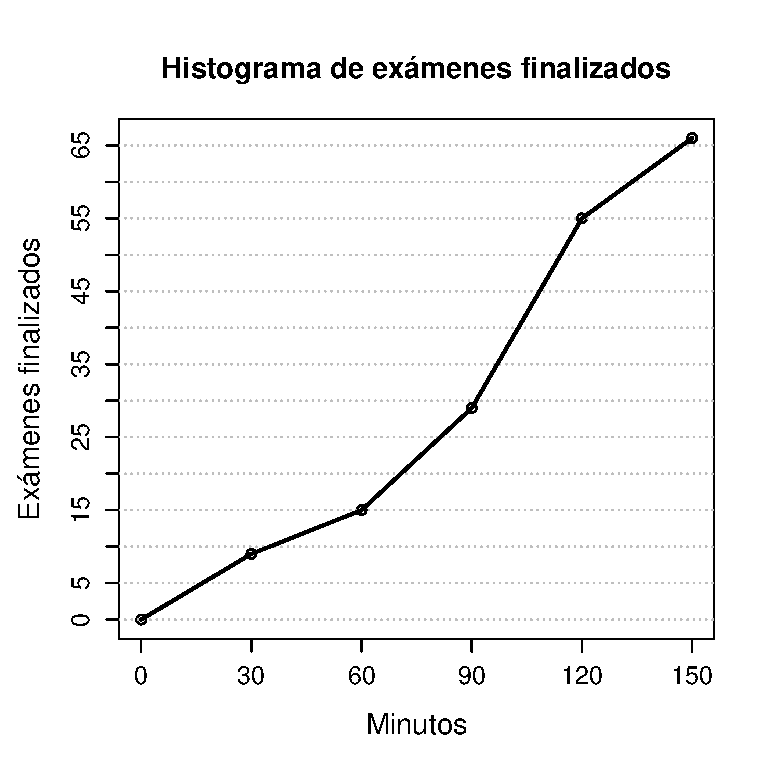
\includegraphics[scale=0.8]{img/poligono-des-56}
\end{center}
Se pide:
\begin{enumerate}
\item ¿Existe mucha dispersión en la muestra? Justificar la respuesta.
\item ¿Cuánto tiempo tiene que pasar para que hayan finalizado el examen la mitad de los alumnos?
\item Estudiar la asimetría de la distribución.  
\end{enumerate}
}
%SOLUCIÓN
{\begin{enumerate}
\item $\bar x= 85.9091$ min, $s^2 =1408.2645$ min$^2$, $s= 37.5268$ min y $cv= 0.4368$, luego existe una dispersión moderada.
\item $Me = 94.6154$ min.
\item $g_1= -0.618$, lo que indica que la distribución es asimétrica hacia la izquierda. 
\end{enumerate}
}
%RESOLUCIÓN
{\begin{enumerate}
\item Para ver si la muestra tienen mucha dispersión hay que calcular la desviación típica o el coeficiente de variación, pero antes necesitamos
conocer las frecuencias absolutas de cada clase. En la tabla que nos dan aparece el número de exámenes finalizados para cada instante, que es,
en realidad, la frecuencia absoluta acumulada. A partir de ella se puede obtener facilmente la frecuencia absoluta de cada clase simplemente
restando a la frecuencia absluta acumulada de la clase siguiente la de la clase actual. Así se obtiene la siguiente tabla de frecuencias. 
\[
\begin{array}{rrrr}
  \hline
 & x_i & n_i & N_i \\ 
  \hline
(0,30] & 15 & 9 & 9 \\ 
  (30,60] & 45 & 6 & 15 \\ 
  (60,90] & 75 & 14 & 29 \\ 
  (90,120] & 105 & 26 & 55 \\ 
  (120,150] & 135 & 11 & 66 \\ 
   \hline
\end{array}\]

Para calcular la desviación típica se añaden nuevas columnas a la tabla de frecuencias con los cálculos necesarios:
\[
\begin{array}{rrrrr}
  \hline
 & x_i & n_i & x_in_i & x_i^2n_i \\ 
  \hline
(0,30] & 15 & 9 & 135 & 2025 \\ 
  (30,60] & 45 & 6 & 270 & 12150 \\ 
  (60,90] & 75 & 14 & 1050 & 78750 \\ 
  (90,120] & 105 & 26 & 2730 & 286650 \\ 
  (120,150] & 135 & 11 & 1485 & 200475 \\ 
  \sum &  & 66 & 5670 & 580050 \\ 
   \hline
\end{array}\]

A partir de la tabla calculamos los estadísticos que se piden:
\begin{align*}
\bar x &= \frac{\sum x_in_i}{n_x} = \frac{5670}{66} = 85.9091,\\
s^2 & = \frac{\sum x_i^2n_i}{n_x}-\bar x^2 = \frac{580050}{66}-7380.3735 = 1408.2645,\\
s & = \sqrt{1408.2645} = 37.5268,\\
cv & = \frac{s}{|\bar x|} = \frac{37.5268}{|85.9091|} = 0.4368.
\end{align*}
Lo que indica que hay una dispersión moderada. 

\item El tiempo que transcurra hasta que hayan finalizado el examen la mitad de los alumnos es precisamente la mediana.
La frecuencia absoluta acumulada correspondiente a la mediana es $66/2 = 33$ de modo que la mediana cae en la clase $[90,120)$, e interpolando en esta clase se obtiene
\[
Me = 90+\frac{33-29}{26}30 = 94.6154 \text{ min}.
\]

\item Para estudiar la asimetría de la muestra se calcula el coeficiente de asimetría. Para ello se añade una nueva columna a la tabla de
frecuencias con las desviaciones a la media al cubo:
\[
\begin{array}{rrrrr}
  \hline
 & x_i & n_i & x_i-\bar x & (x_i-\bar x)^3n_i \\ 
  \hline
(0,30] & 15 & 9 & -70.9091 & -3208841.4726 \\ 
  (30,60] & 45 & 6 & -40.9091 & -410781.3674 \\ 
  (60,90] & 75 & 14 & -10.9091 & -18175.8077 \\ 
  (90,120] & 105 & 26 & 19.0909 & 180906.0856 \\ 
  (120,150] & 135 & 11 & 49.0909 & 1301355.3719 \\ 
  \sum &  & 66 &  & -2155537.1901 \\ 
   \hline
\end{array}\]

A partir de la tabla calculamos los estadísticos que se piden:
\[
g_{1} &= \frac{\sum (x_i-\bar x)^3 n_i/n_x}{s_x^3} = \frac{-2155537.1901/66}{37.5268^3} = -0.618.
\]

Lo que indica que la distribución es asimétrica hacia la la izquierda. 
\end{enumerate}
}

